% should I use value functions or expected cost functions

\def\year{2016}
\documentclass[letterpaper]{article}
\usepackage{aaai}
\usepackage{times}
\usepackage{helvet}
\usepackage{courier}
\frenchspacing
%\setlength{\pdfpagewidth}{8.5in}
%\setlength{\pdfpageheight}{11in}

\usepackage{amsmath}%
\usepackage{amsfonts}%
\usepackage{amssymb}%
\usepackage{graphicx}
\usepackage{url}
\usepackage{subfigure}
\usepackage{color}

\usepackage{epstopdf}
\usepackage{color}
\usepackage{listings}
\usepackage{multicol}
\usepackage{multirow}
\usepackage{tikz}
\usepackage{hyperref}
\usepackage{booktabs}
\usepackage{mathtools}
\usepackage[capitalise,noabbrev]{cleveref}
\DeclareGraphicsRule{.tif}{png}{.png}{`convert #1 `dirname #1`/`basename #1 .tif`.png}
\graphicspath{{../TRB_paper/plots/}{plots/}}

\setcounter{secnumdepth}{2}


\usepackage[inline]{enumitem}  %% For in-line lists


\newcommand{\Omit}[1]{}


% CITATIONS
%------------------------------------------
% TRB uses an Author (num) citation style. I haven't found a way to make
% LaTeX/Bibtex do this automatically using the standard \cite macro, but
% this modified \trbcite macro does the trick.

% SCOTT CHANGED MACROS TO USE AAAI CITATIONS

%% sort&compress option?
%%\usepackage[sort,numbers]{natbib}
%%	\newcommand{\trbcite}[1]{\citeauthor{#1} ({\it \citenum{#1}})}
%%	\newcommand{\trbcitenum}[1]{({\it \citenum{#1}})}
%%\setcitestyle{round}
\newcommand{\trbcite}[1]{\citeauthor{#1} (\citeyear{#1})}
\newcommand{\trbcitenum}[1]{\cite{#1}}


%% Toggle comments on next two lines to turn on/off editorial remarks
\newcommand{\remark}[1]{\color{red} #1 \color{black}}
\newcommand{\fnremark}[1]{\remark{\footnote{\remark{#1}}}}
\newcommand{\toIain}[1]{\footnote{\textbf{To Iain}: #1}}
\newcommand{\toFelipe}[1]{\footnote{\textbf{To Felipe}: #1}}
\newcommand{\comment}[1]{}

%% FWT: I'm using this to highlight parts of the text that might need polishing.
\newcommand{\authorHighlight}[1]{\textcolor{red}{#1}}


%%
%% Final version: Uncomment the lines bellow to turn off all the high-lights and
%% other remarks
%%
\renewcommand{\remark}[1]{}
\renewcommand{\fnremark}[1]{}
\renewcommand{\toIain}[1]{}
\renewcommand{\toFelipe}[1]{}
\renewcommand{\comment}[1]{}
\renewcommand{\authorHighlight}[1]{#1}


%\renewcommand{\authorHighlight}[1]{#1}

% All math definitions before start document
%% Adds the command \xspace to be used in \newcommand and automatically decide
%% whenever to add a space after the command
\usepackage{xspace}

% Queue marks for the different traffic inflow explanation
\newcommand{\qLowTraf}{\ensuremath{\diamondsuit}\xspace}
\newcommand{\qHighTraf}{\ensuremath{\clubsuit}\xspace}
\newcommand{\qVarTraf}{\ensuremath{\spadesuit}\xspace}

\newcommand{\Vol}{\ensuremath{V}\xspace}
\newcommand{\Matrix}[1]{\ensuremath{\mathbf{#1}}}
\newcommand{\Vector}[1]{\ensuremath{\vec{#1}}}


\newcommand{\Net}{\ensuremath{\mathcal{N}}\xspace}
\newcommand{\Qset}{\ensuremath{\mathcal{Q}}\xspace}
\newcommand{\QPset}[1]{\ensuremath{\mathcal{Q}_{#1}^{\mathcal{P}}}}
\newcommand{\Lset}{\ensuremath{\mathcal{L}}\xspace}
\newcommand{\Pset}{\ensuremath{\mathcal{P}}\xspace}
\newcommand{\Pvec}{\ensuremath{\Vector{P}}\xspace}
\newcommand{\Fvec}{\ensuremath{\Vector{F}}}
\newcommand{\Prvec}{\ensuremath{\Vector{Pr}}}
\newcommand{\fvec}[1]{\ensuremath{\mathbf{f}_{#1}}}
\newcommand{\tl}{\ensuremath{\ell}\xspace}

% Uncomment for old style equations
%\newcommand*{\oldeq}{}

% Uncomment for new style equations with Lin and Wang subscripts
\newcommand*{\neweqsub}{}

% Uncomment for new in out flow variables
\newcommand*{\newinoutflow}{}

\ifdefined\oldeq
%
% Old style equations
%
\newcommand{\q}[2][n]{\ensuremath{q_{#2}^{#1}}}
\newcommand{\qin}[2][n]{\ensuremath{q_{#2,in}^{#1}}}
\newcommand{\qout}[2][n]{\ensuremath{q_{#2,out}^{#1}}}
\newcommand{\f}[3][n]{\ensuremath{f_{#2,#3}^{#1}}}
\newcommand{\inq}[2][n]{\ensuremath{in_{#2}^{#1}}}
\newcommand{\outq}[2][n]{\ensuremath{out_{#2}^{#1}}}
\newcommand{\p}[3][n]{\ensuremath{p_{#2,#3}^{#1}}}
\newcommand{\pd}[3][n]{\ensuremath{d_{#2,#3}^{#1}}}
\newcommand{\aph}[2][n]{\ensuremath{\alpha_{#2}^{#1}}}
\newcommand{\tn}[1][n]{\ensuremath{t^{#1}}}
\newcommand{\DT}[1][n]{\ensuremath{\Delta t^{#1}}}

\newcommand{\Nn}{\ensuremath{\mathrm{N}}\xspace}
\newcommand{\Qn}{\ensuremath{|\mathcal{\Qset}|}\xspace}
\newcommand{\Ln}{\ensuremath{|\mathcal{\Lset}|}\xspace}
\newcommand{\Pn}[1][\ell]{\ensuremath{|\mathcal{\Pset}_{#1}|}}
\newcommand{\TMAX}{\ensuremath{T^{MAX}}\xspace}
\newcommand{\QMAX}[1]{\ensuremath{Q_{#1}^{MAX}}}
\newcommand{\QIN}[1]{\ensuremath{Q_{#1}^{IN}}}
\newcommand{\QOUT}[1]{\ensuremath{Q_{#1}^{OUT}}}
\newcommand{\QDELAY}[1]{\ensuremath{Q_{#1}^{DELAY}}}
\newcommand{\FMAX}[2]{\ensuremath{F_{#1,#2}^{MAX}}}
\newcommand{\FTURN}[2]{\ensuremath{F_{#1,#2}^{TURN}}}
\newcommand{\PTMAX}[2]{\ensuremath{PT_{#1,#2}^{MAX}}}
\newcommand{\PTMIN}[2]{\ensuremath{PT_{#1,#2}^{MIN}}}
\newcommand{\CTMAX}[1]{\ensuremath{CT_{#1}^{MAX}}}
\newcommand{\CTMIN}[1]{\ensuremath{CT_{#1}^{MIN}}}

\else
\ifdefined\neweqsub
%
% New style equations subscript
%
\newcommand{\q}[2][n]{\ensuremath{q_{#2,#1}}}
\newcommand{\qin}[2][n]{\ensuremath{q_{#2,#1}^{\mathrm{in}}}}
\newcommand{\qstop}[2][n]{\ensuremath{q_{#2,#1}^{\mathrm{stop}}}}
\newcommand{\qout}[2][n]{\ensuremath{q_{#2,#1}^{\mathrm{out}}}}
\newcommand{\f}[3][n]{\ensuremath{f_{#2,#3,#1}}}

\ifdefined\newinoutflow
\newcommand{\inq}[2][n]{\ensuremath{f^\mathrm{in}_{#2,#1}}}
\newcommand{\outq}[2][n]{\ensuremath{f^\mathrm{out}_{#2,#1}}}
\else
\newcommand{\inq}[2][n]{\ensuremath{in_{#2,#1}}}
\newcommand{\outq}[2][n]{\ensuremath{out_{#2,#1}}}
\fi

\newcommand{\p}[3][n]{\ensuremath{p_{#2,#3,#1}}}
\newcommand{\pd}[3][n]{\ensuremath{d_{#2,#3,#1}}}
\newcommand{\aph}[2][n]{\ensuremath{\alpha_{#2,#1}}}
\newcommand{\tn}[1][n]{\ensuremath{t_{#1}}}
\newcommand{\DT}[1][n]{\ensuremath{\Delta t_{#1}}}
\newcommand{\vecDT}{\ensuremath{\Vector{\Delta t}}\xspace}

\newcommand{\Nn}{\ensuremath{\mathrm{N}}\xspace}
\newcommand{\Qn}{\ensuremath{|\mathcal{\Qset}|}\xspace}
\newcommand{\Ln}{\ensuremath{|\mathcal{\Lset}|}\xspace}
\newcommand{\Pn}[1][\ell]{\ensuremath{|\mathcal{\Pset}_{#1}|}}
\newcommand{\TMAX}{\ensuremath{\mathrm{T}}\xspace}
\newcommand{\QMAX}[1]{\ensuremath{\mathrm{Q}_{#1}}}

\ifdefined\newinoutflow
%\newcommand{\QIN}[1]{\ensuremath{\mathrm{F}_{in\shortrightarrow#1}}}
%\newcommand{\QOUT}[1]{\ensuremath{\mathrm{F}_{#1\shortrightarrow out}}}
%\newcommand{\QIN}[1]{\ensuremath{\mathrm{F}_{#1}^{\mathrm{in}}}}
\newcommand{\MatQIN}{\ensuremath{\Matrix{I}}\xspace}
\newcommand{\QIN}[2]{\ensuremath{I_{#1,#2}}}
\newcommand{\QOUT}[1]{\ensuremath{\mathrm{F}_{#1}^{\mathrm{out}}}}
\else
\newcommand{\QIN}[1]{\ensuremath{\mathrm{Q}_{#1}^{\mathrm{in}}}}
\newcommand{\QOUT}[1]{\ensuremath{\mathrm{Q}_{#1}^{\mathrm{out}}}}
\fi

\newcommand{\QDELAY}[1]{\ensuremath{\mathrm{T}_{#1}^{\mathrm{prop}}}}
\newcommand{\FMAX}[2]{\ensuremath{\mathrm{F}_{#1,#2}}}
\newcommand{\FTURN}[2]{\ensuremath{\mathrm{Pr}_{#1,#2}}}
\newcommand{\PTMAX}[3][,]{\ensuremath{\mathrm{\Phi}_{#2#1#3}^{\mathrm{max}}}}
\newcommand{\PTMIN}[3][,]{\ensuremath{\mathrm{\Phi}_{#2#1#3}^{\mathrm{min}}}}
\newcommand{\VecPTMAX}[1]{\ensuremath{\Vector{\mathrm{\Phi}}_{#1}^{\mathrm{max}}}}
\newcommand{\VecPTMIN}[1]{\ensuremath{\Vector{\mathrm{\Phi}}_{#1}^{\mathrm{min}}}}
\newcommand{\CTMAX}[1]{\ensuremath{\mathrm{\Psi}_{#1}^{\mathrm{max}}}}
\newcommand{\CTMIN}[1]{\ensuremath{\mathrm{\Psi}_{#1}^{\mathrm{min}}}}



\else
%
% New style equations superscript
%
\newcommand{\q}[2][n]{\ensuremath{q_{#2}^{(#1)}}}
\newcommand{\qin}[2][n]{\ensuremath{q_{#2,in}^{(#1)}}}
\newcommand{\qstop}[2][n]{\ensuremath{q_{#2,stop}^{(#1)}}}
\newcommand{\qout}[2][n]{\ensuremath{q_{#2,out}^{(#1)}}}
\newcommand{\f}[3][n]{\ensuremath{f_{#2\to#3}^{(#1)}}}
\newcommand{\inq}[2][n]{\ensuremath{in_{#2}^{(#1)}}}
\newcommand{\outq}[2][n]{\ensuremath{out_{#2}^{(#1)}}}
\newcommand{\p}[3][n]{\ensuremath{p_{#2,#3}^{(#1)}}}
\newcommand{\pd}[3][n]{\ensuremath{d_{#2,#3}^{(#1)}}}
\newcommand{\aph}[2][n]{\ensuremath{\alpha_{#2}^{(#1)}}}
\newcommand{\tn}[1][n]{\ensuremath{t^{(#1)}}}
\newcommand{\DT}[1][n]{\ensuremath{\Delta t^{(#1)}}}

\newcommand{\Nn}{\ensuremath{\mathrm{N}}\xspace}
\newcommand{\Qn}{\ensuremath{|\mathcal{\Qset}|}\xspace}
\newcommand{\Ln}{\ensuremath{|\mathcal{\Let}|}\xspace}
\newcommand{\Pn}[1][\ell]{\ensuremath{|\mathcal{\Pet}_{#1}|}}
\newcommand{\TMAX}{\ensuremath{\mathrm{T}}\xspace}
\newcommand{\QMAX}[1]{\ensuremath{\mathrm{Q}_{#1}}}
\newcommand{\QIN}[1]{\ensuremath{\mathrm{Q}_{#1}^{\mathrm{in}}}}
\newcommand{\QOUT}[1]{\ensuremath{\mathrm{Q}_{#1}^{\mathrm{out}}}}
\newcommand{\QDELAY}[1]{\ensuremath{\mathrm{Q}_{#1}^{\mathrm{delay}}}}
\newcommand{\FMAX}[2]{\ensuremath{\mathrm{F}_{#1\to#2}}}
\newcommand{\FTURN}[2]{\ensuremath{\mathrm{Pr}_{#1\to#2}^{\mathrm{}}}}
\newcommand{\PTMAX}[3][,]{\ensuremath{\mathrm{\Phi}_{#2#1#3}^{\mathrm{max}}}}
\newcommand{\PTMIN}[3][,]{\ensuremath{\mathrm{\Phi}_{#2#1#3}^{\mathrm{min}}}}
\newcommand{\CTMAX}[1]{\ensuremath{\mathrm{\Psi}_{#1}^{\mathrm{max}}}}
\newcommand{\CTMIN}[1]{\ensuremath{\mathrm{\Psi}_{#1}^{\mathrm{min}}}}

\fi



%% Macros for constraints
\newcounter{constraintcounter}
% Use \tagconstrain{labelName} to tag the constraint as C.X and label
% it as labelName
\newcommand{\tagconstrain}[1]{\refstepcounter{constraintcounter}\tag{C\theconstraintcounter}\label{#1}}
% Use the cAlign as the align environment for constraint
\newenvironment{cAlign}{\align}{\endalign}
% defining the name for the labels of the type cAlign
\crefname{equation}{constraint}{constraints}

%%%%%%%%%%%%%%%%%%%%%%%%%%%%%%%%%%%%%%%%%%%%%%%%%%%%%%%%%%%%%%%%%%%%%%%%%%%%%%
%%
%%                                  SPACING
%%
%%                       Preventing widow/orphan lines
%% tex.stackexchange.com/questions/4152/how-do-i-prevent-widow-orphan-lines
%%
\widowpenalty=10000
\clubpenalty=10000
%%
%%
%%     Preventing inline equations to be broken (and possibly more stuff)
%% http://tex.stackexchange.com/a/94397
%%
\binoppenalty=\maxdimen
\relpenalty=\maxdimen
%%
%%
%%                     Changing the spacing between lines
%%
%\usepackage{setspace}  %% \begin{singlespace} \begin{doublespace}, etc
%\newcommand{\fwtBodySpacing}{\setstretch{1.235}}
%\setstretch{1.22} % 1.235 is almost the same as \onehalfspacing
%\newcommand{\fwtRegularSpacing}{\setstrech{1}}
%%\onehalfspacing
%%
%%
%%                   EXPLICITLY CHANGING INTERWORD SPACING
%%
%% See: http://tex.stackexchange.com/questions/23921/how-to-shorten-shrink-spaces-between-words
%%
%% To see the current spacing add this to the text
%% \the\fontdimen2\font
%%
%% If the first parameter is 0, then it disables the change. Good for testing
%% the effects of it
\newcommand{\changeInterWordSpace}[3]{\ifthenelse{#1 = 0}{#3}{\changeInterWordSpaceREAL{#2}{#3}}}
%%
\newcommand*{\changeInterWordSpaceREAL}[2]{%
\newdimen\origiwspc%
%\newdimen\origiwstr%
\origiwspc=\fontdimen2\font% original inter word space
%\origiwstr=\fontdimen2\font% original inter word stretch
\fontdimen2\font=#1% inter word space
%\fontdimen3\font=0.1em%
#2%
\fontdimen2\font=\origiwspc% (original) inter word space
%\fontdimen3\font=\origiwstr% (original) inter word stretch
}
%%%%%%%%%%%%%%%%%%%%%%%%%%%%%%%%%%%%%%%%%%%%%%%%%%%%%%%%%%%%%%%%%%%%%%%%%%%%%%



\begin{document}

\title{A Novel Mixed Integer LP Model to\\ Mitigate
 the Impact of Light Rail on Conventional Traffic Networks}

\author{Paper ID 68}
\Omit{
\author{
Iain Guilliard \and Felipe Trevizan\\
\small Machine Learning Group, NICTA\\
\small Research School of Computer Science, ANU\\
\small iain.guilliard@nicta.com.au\\
\small felipe.trevizan@nicta.com.au\\
\And Scott Sanner\\
\small Computer Science Department\\
\small Oregon State University\\ 
\small scott.sanner@oregonstate.edu\\
\And Brian Williams\\
\small MERS Group\\
\small Computer Science and AI Laboratory\\
\small MIT\\
\small williams@mit.edu\\
}
}
\date{}

\maketitle

\begin{abstract}
\section*{Abstract}

% Basically just the topic sentences of the Intro. :)  < 250 words

% Motivation, quantify

As urban traffic congestion is on the increase worldwide, it is
critical to maximize capacity and throughput of existing road
infrastructure through optimized traffic signal control.  To this end,
we build on the body of work in mixed integer linear programming
(MILP) approaches that attempt to jointly optimize traffic signal
control over an entire traffic network and specifically on
improving the scalability of these methods for large numbers of
intersections.  Our primary insight in this work stems from the fact
that MILP-based approaches to traffic control used in a receding
horizon control manner (that replan at fixed time intervals) need to
compute high fidelity control policies only for the early stages of
the signal plan; therefore, coarser time steps can be employed to
``see'' over a long horizon to preemptively adapt to distant platoons
and other predicted long-term changes in traffic flows.  To this end,
we contribute the queue transmission model (QTM) which blends elements
of cell-based and link-based modeling approaches to enable a
non-homogeneous time MILP formulation of traffic signal control.
%
We then experiment with this novel QTM-based MILP control in a range
of traffic networks and demonstrate that the non-homogeneous MILP
formulation achieves (i) substantially lower delay solutions, (ii)
improved per-vehicle delay distributions, and (iii) more optimal travel
times over a longer horizon in comparison to the homogeneous MILP
formulation with the same number of binary and continuous variables.
%% WORD COUNT: the above is approximately 232 words

%demonstrating that using non-homogeneous time steps, we can
%optimally solve large networks with a fraction of the MILP binary
%variables required to achieve the same solution quality with a
%homogeneous time step.
%
%demonstrating substantially improved scalability and
%traffic signal control quality when using non-homogeneous time steps
%in comparison to homogeneous time steps.
%
%
%Since the number of binary variables has a large impact on MILP solving efficiency, 
%reducing the number of binary variables is critical for scalability of MILP-based
%traffic signal control solutions.

%
%% I think the following statement I wrote is too risky to say given that
%% - the traffic withholding problem may occur
%% - we are using the major/minor frame approach
%% - we are somehow claiming that the QTM is an accurate model of real traffic flow
%% - Gurobi may have a time-limit for some results
%Our experiments also provide near-optimal traffic control policies
%for dense traffic networks up to nine intersections than shown in previous
%implementations of MILP-based traffic signal control.


%\newcommand{\wordsInAbstract}{
    \immediate\write18{texcount -sum -1 tex/Abstract.tex > 'countInAbstract.txt'}
    \IfFileExists{./countInAbstract.txt}{\input{countInAbstract.txt}}{??}}
\fnremark{Using \wordsInAbstract{} words up to here. Maximum is 250 words.

Make sure to follow instructions and author guide:
  \url{http://onlinepubs.trb.org/onlinepubs/AM/InfoForAuthors.pdf}
  \url{http://onlinepubs.trb.org/onlinepubs/am/2015/WritingForTheTRRecord.pdf}

Also note this example related paper from Steve Smith (formatted to TRB specs):
  \url{https://www.ri.cmu.edu/pub_files/2014/1/TRB14UTC.pdf}
}

 
\end{abstract}



% Note: in Steve Smith's TRB article, Intro on numbered page 2, so this seems OK
\section{Introduction}

As urban traffic congestion is on the increase worldwide with
estimated productivity losses in the hundreds of billions of dollars
in the U.S. alone and immeasurable environmental
impact~\cite{bazzan2013intro}, many cities are increasingly looking to
inexpensive public transit options such as light rail in
order to reduce the number of conventional traffic commuters.  Since
light rail often operates at street-level and requires coordination
with conventional traffic networks and signal control, a major concern
in light rail installation is whether enough commuters will switch to
it to offset the additional constraints it places on traffic signal
control.  Unfortunately, many large cities still use some degree of
\emph{fixed-time} control~\trbcitenum{el2013multiagent}.  As we show
in this paper, conventional fixed-time control methods pose
significant challenges for the integration of light rail even when
their timings are optimized to synchronize with the light rail
schedule.

However, there is further opportunity to improve traffic signal
control through the use of \emph{optimized adaptive} controllers based
on mixed integer (linear)
programming~\trbcitenum{gartner1974optimization,gartner2002arterial,lo1998novel,he2011pamscod,lin2004enhanced,han2012link}.
To this end, we develop a linear programming model of traffic flow
termed the {\it Queue Transmission Model (QTM)} where traffic signals
can be represented as discrete variables, light rail schedules can be
represented as traffic signal constraints, and Mixed Integer Linear
Programming (MILP) can be used to optimize the traffic signals to
minimize delay subject to the light rail constraints.  As we show in
this paper, such controllers hold the promise of maximizing existing
infrastructure capacity by finding optimized traffic signal control
policies that are tightly integrated with light rail transit schedules
to mitigate the impact of the latter on conventional traffic delays.

Overall, our key results in this paper show that while there is a
substantial impact of light rail on conventional vehicle traffic delay
using popular fixed-time signal control, our novel optimized signal
control virtually nullifies this impact. Ultimately this leads to a
win-win situation where both conventional vehicle traffic and light
rail commuters benefit through the application of MILP-based
optimization to jointly manage public transit and conventional traffic
networks.

\Omit{
%master-slave approaches such as SCATS and SCOOT, such optimized methods
However, optimized methods are computationally demanding 
%compared to adpative control methods such as SCOOT and SCATS
%(which can run on 1970's error hardware)
and often do not guarantee \emph{jointly} optimal solutions over a
large intersection network either because (a) they only consider
coordination of neighboring intersections or arterial routes or (b)
they fail to scale to large intersection networks simply for
computational reasons.  We remark that the latter scalability issue is endemic
to many mixed integer programming approaches to optimized signal control.

In this work, we build on the body of work in mixed integer linear
programming (MILP) approaches that attempt to jointly optimize traffic
signal control over an \emph{entire traffic network}~(rather than
focus on arterial routes) and specifically on improving the
scalability of these methods for large urban traffic networks.  In our
investigation of existing approaches in this vein, namely exemplar
methods in the spirit of~\trbcitenum{lo1998novel,lin2004enhanced,han2012link} that
use a (modified) cell transmission model
(CTM)~\trbcitenum{daganzo1994cell,daganzo1995cell} for their underlying
prediction of traffic flows, we remark that a major drawback is the
CTM-imposed requirement to choose a predetermined \emph{homogeneous} (and
often necessarily small) time step for reasonable modeling fidelity.
This need to model a large number of CTM cells with a small time step
leads to MILPs that are exceedingly large and often intractable to
solve. %% FWT: seems redundant "for large traffic networks."

Our primary insight in this work stems from the fact that MILP-based
approaches to traffic control used in a receding horizon control
manner (that replan at fixed time intervals) need to compute high
fidelity control policies only for the early stages of the signal
plan; therefore, coarser time steps can be employed to ``see'' over a
long horizon to preemptively adapt to distant platoons and other
predicted long-term changes in traffic flows.
This need for non-homogeneous control in
turn spawns the need for an additional innovation: we require a
traffic flow
%% FWT: "simulation" here is confusing in my opinion.
model that permits non-homogeneous time steps and properly models the
travel time delay between lights.  To this end, we might consider CTM
extensions such as the variable cell length
CTM~\trbcitenum{xiaojian2010urban}, stochastic CTM
~\trbcitenum{sumalee2011stochastic,jabari2012stochastic},
CTM extensions for better modeling freeway-urban
interactions~\trbcitenum{huang2011traffic} including CTM hybrids with
link-based models~\trbcitenum{muralidharan2009freeway}, assymmetric
CTMs for better handling flow imbalances in merging
roads~\trbcitenum{gomes2006optimal}, the situational CTM for better
modeling of boundary conditions~\trbcitenum{kim2002online}, and the
lagged CTM for improved modeling of the flow density
relation~\trbcitenum{lu2011discrete}.  However, despite the widespread
varieties of the CTM and usage for a range of
applications~\trbcitenum{alecsandru2011assessment}, there seems to be
no extension that permits \emph{non-homogeneous} time steps as proposed in
our novel MILP-based control approach.

\begin{figure*}[t!]
\centering
%  trim={<left> <lower> <right> <upper>}
\subfigure[]{
\label{subfig:overlay}
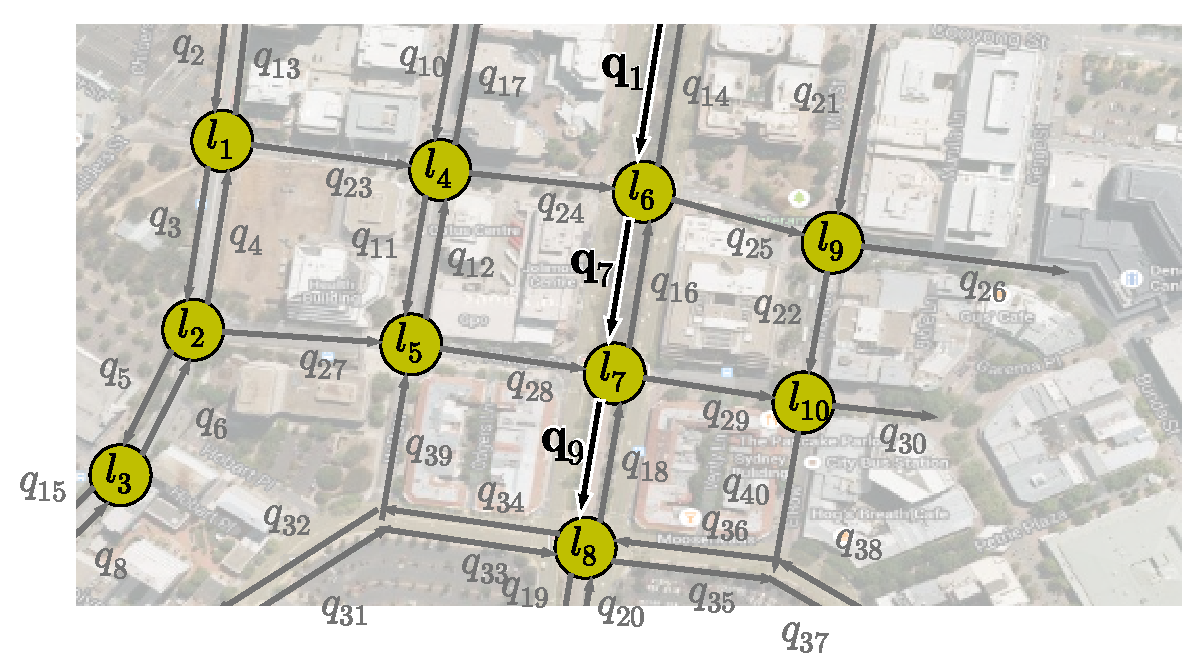
\includegraphics[width=0.5\textwidth,trim={1.3cm 1.1cm 3cm 0.5cm},clip]{map_overlay.pdf}}
\subfigure[]{
\label{subfig:example}
%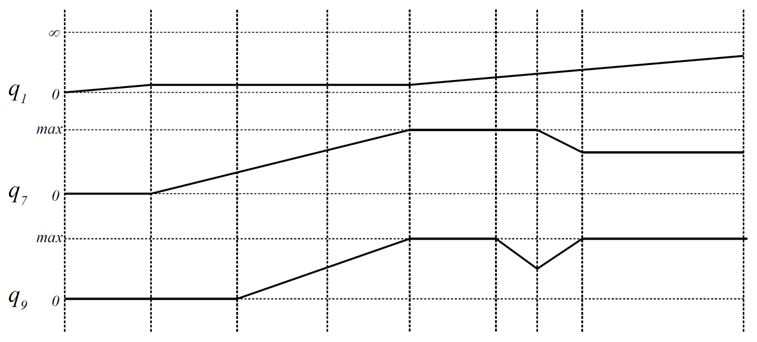
\includegraphics[width=0.45\textwidth,trim={0cm 0cm 0cm 0cm},clip]{map_example.png}
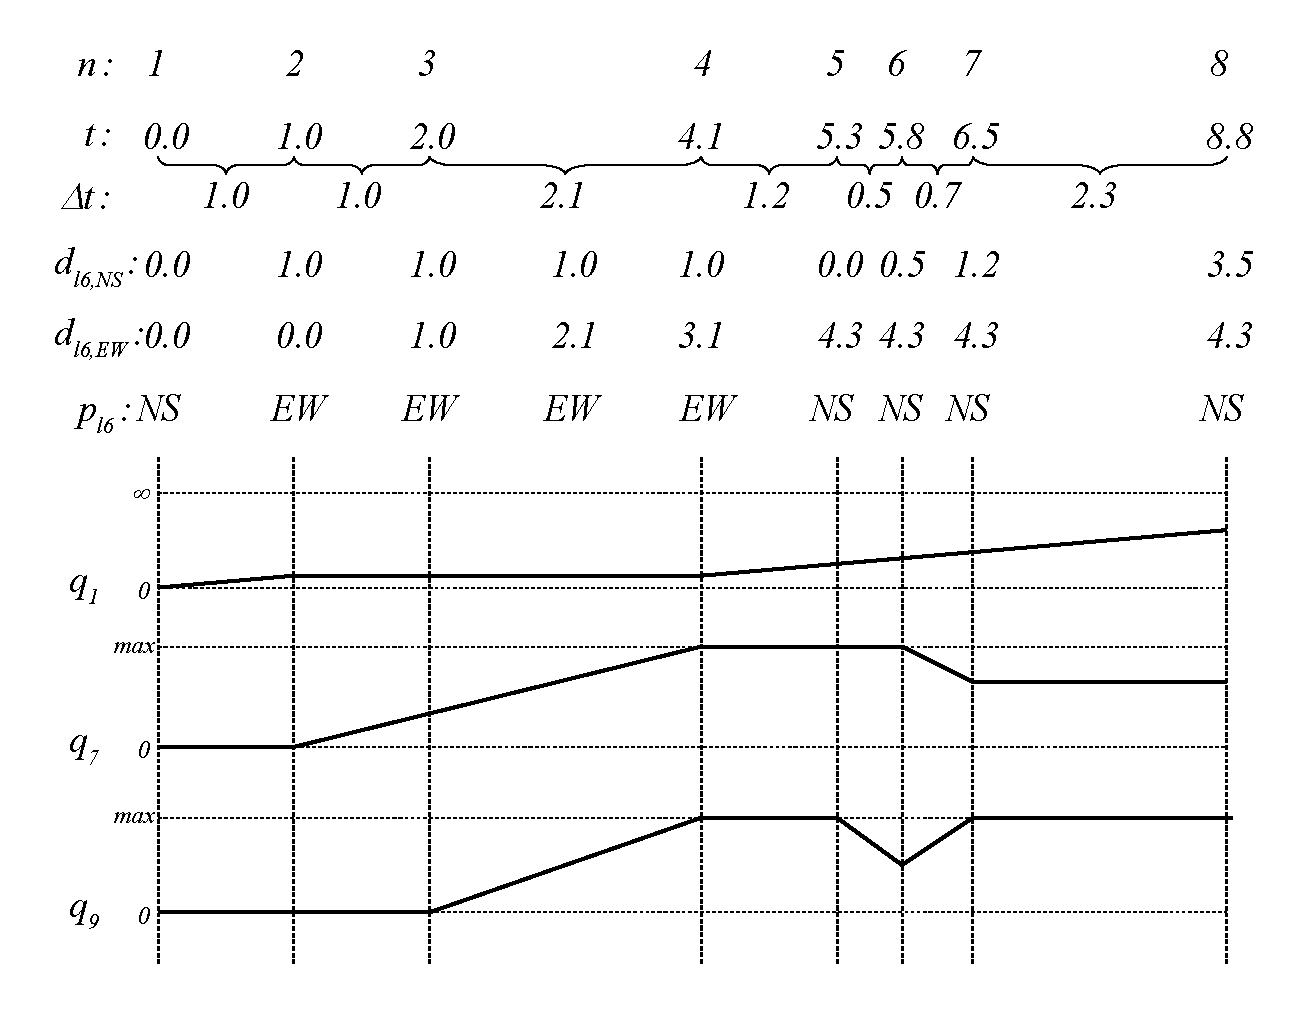
\includegraphics[width=0.44\textwidth,trim={0cm 0cm 0cm 0cm},clip]{pw_queues.pdf}
}
% NOTE: Reviewers like to skim a paper by reading captions so I intentionally
\caption{(a) Example of a real traffic network modeled using the
  QTM. (b) A preview of different QTM model parameters as a function
  of \emph{non-homogeneous} discretized time intervals indexed by $n$.
  For each $n$, we show the following parameters: the elapsed time
  $t$, the non-homogeneous time step length $\Delta t$, the cumulative
  duration $d$ of two different light phases for $l_6$, the phase $p$
  of light $l_6$, and the traffic volume of different queues $q$
  linearly interpolated between time points.  There is technically a
  binary $p$ for each phase, but we abuse notation and simply
  show the current active phase: $\mathit{NS}$ for \emph{north-south green} and 
  $\mathit{EW}$ for \emph{east-west green} assuming the top of the map is north.
  Here we see that traffic progresses from $q_1$ to $q_7$ to $q_9$
  according to light phases and traffic propagation delay with non-homogeneous time steps
  only at required changepoints.
  %Time interval boundaries are only necessary at
  %nonlinear changepoints in queue volume.
  We refer to the QTM model section for
  precise notation and technical definitions.}
\label{fig:qtm}
%
\end{figure*}}

\Omit{
For this reason, as a major contribution of this work to enable our
non-homogeneous time MILP-based model of joint intersection control, we
contribute the queue transmission model (QTM) that blends elements of
cell-based and link-based modeling approaches as illustrated
and summarized in Figure~\ref{fig:qtm}.  The QTM offers the following key benefits:
\begin{itemize}
%
\item  Unlike previous CTM-based joint intersection signal 
  optimization~\trbcitenum{lo1998novel,lin2004enhanced,han2012link}, the QTM is
  intended for \emph{non-homogeneous} time steps that can
  be used for control over large horizons.
%
\item Any length of roadway without merges or diverges can be modeled
  as a single queue leading to compact QTM MILP encodings of large traffic
  networks 
  (i.e., large numbers of cells and their associated MILP variables are
  not required \emph{between} intersections).
%
\item The QTM accurately models fixed travel time delays critical to green wave
  coordination as
  in~\trbcitenum{gartner1974optimization,gartner2002arterial,he2011pamscod}
  through the use of a non-first order Markovian update model and further combines this
  with fully joint intersection signal optimization in the spirit 
  of~\trbcitenum{lo1998novel,lin2004enhanced,han2012link}.
\end{itemize}

In the remainder of this paper, we first formalize our
novel QTM model of traffic flow with non-homogeneous time steps and
show how to encode it as a linear program for computing traffic flows.
%
Next we proceed to allow the traffic signals to become discrete phase
variables that are optimized subject to a delay minimizing objective
and standard minimum and maximum time constraints for cycles and
phases; this results in our final MILP formulation of traffic signal
control.
%
We then experiment with this novel QTM-based MILP control in a range
of traffic networks and demonstrate that the non-homogeneous MILP
formulation achieves (i) substantially lower delay solutions, (ii)
improved per-car delay distributions, and (iii) more optimal travel
times over a longer horizon in comparison to the homogeneous MILP
formulation with the same number of binary and continuous variables.
}

%demonstrating that using non-homogeneous time steps, we can
%optimally solve large networks with a fraction of the MILP binary
%variables required to achieve the same solution quality with a
%homogeneous time step.
%
%We then experiment with this novel QTM-based MILP signal control in a range
%of traffic networks demonstrating substantially improved scalability and
%traffic signal control quality when using non-homogeneous time steps
%in comparison to homogeneous time steps.
%
%We then experiment with this novel QTM-based MILP control in
%a range of networks demonstrating the improved scalability possible
%with non-homogeneous time steps in comparison to homogeneous
%time steps.
%
%These experiments also provide near-optimal traffic control policies
%for larger horizons and larger networks than shown in previous
%implementations of MILP-based traffic signal control.
%\fnremark{ We could really use some pictures in the Intro to refer to
%  here and subsequently -- both a traffic network divided into queues,
%  and the concept of the piecewise linear evolution of traffic flow
%  with {\bf non-homogeneous} (dilated) time steps, something like I had
%  provided in my early writeup.  I think these help visually explain
%  much of the context for the paper and its approach and are critical
%  for reviewer understanding on a time budget for reading this They
%  may only read the first 2-3 pages and then skim!}
%\fnremark{A picture is worth
%  a 1000 words but we only pay 250, hence a 4X ROI on pictures!}

%%%%%%%%%%%%%%%%%%%%%%%%%%%%%%%%%%%%%%%%%%%%%%%%%%%%%%%%%%%%%%%%%%%%%%%%%%
%%%%%%%%%%%%%%%%%%%%%%%%%%%%%%%%%%%%%%%%%%%%%%%%%%%%%%%%%%%%%%%%%%%%%%%%%%
%%%%%%%%%%%%%%%%%%%%%%%%%%%%%%%%%%%%%%%%%%%%%%%%%%%%%%%%%%%%%%%%%%%%%%%%%%

\comment{
optimization techniques as
proposed in various works~\cite (Gartner, Lin and Wang, MARLIN --
Toronto, SURTRAC -- Smith).  In this work, we specifically build on
the MILP approach to traffic optimization that extends previous work
by Lin and Wang who optimize traffic signals (discrete choices at each
time step) in a Cell Transmission Model
(CTM)~\trbcite{daganzo1995cell} of traffic flow.  Unfortunately a CTM
based model is limited in scalability by the requirement that each
road way in the network must be partitioned up into segments that take
exactly $\DT[]=1$ to traverse at the free flow speed.  This leads to a
large number of cells (and hence variables in the MILP) and it makes
it difficult to allow for variable length (non-homogeneous) time steps
in the model updates that we demonstrate in this work to be useful for
optimized traffic signal planning over long horizons.

To allow for more parsimonious models of traffic flow and non-homogeneous
time steps for updates, we introduce the queue transmission model (QTM) [succinct description needed], which offers the following
benefits:
\begin{itemize}
\item non-homogeneous time steps which can keep the model compact over long horizons
\item models platoons without fine-grained cell-based road model or explicit variables to model platoons -- underlies a key precept in urban traffic control to let platoons pass through without stopping,
\item still leads to a MILP, albeit one with much fewer variables owing to the reduced number of queues vs. cells and the reduced number of time steps.
\end{itemize}
Some drawbacks -- does not capture nonlinear flow-density relationship of the
fundamental diagram.  \remark{Argue why this is OK for saturated
  urban networks at peak times.  Green waves in SCATS/SCOOT operate on
  principle of a fixed propagation time, so does Gartner's MILP model.
Captures the right level of detail without blowing up size of model.}
}

%%%%%%%%%%%%%%%%%%%%%%%%%%%%%%%%%%%%%%%%%%%%%%%%%%%%%%%%%%%%%%%%%%%%%%%%%%

\comment{
Lin and Wang aim for network-wide control with a MILP but use
a CTM that requires the time-step to be fixed (otherwise changing
time steps would lead to changing cell sizes and require
dynamic traffic realllocation).

Other GA and reinforcement learning methods, but hard to provide
optimality guarantees.

Much work on optimized traffic control focusing on green-wave
signal coordination given predicted demands and are 
non-homogeneous, but these are largely focused on arterial
control.

Need a deep lookahead possible with non-homogeneous time steps,
but a globally optimized model.  Need to move beyond CTM of
Lin and Wang since this requires fixed time steps, but
still need to model coordination and delays.


Many extensions of CTM for various settings.
...
However, none of these allow non-homogeneous modeling.


To this end we introduce the QTM.  Shares aspects of link-based 
and cell-based models while getting delays right (as in existing
MILP control methosd), but allowing for non-homogeneous time
steps, unlike existing CTMs or extensions.  Ultimately we
will show that a non-homogeneous time step leads to smaller MILPs
and hence improved scalability over a fixed homogeneous time
variant.
}

%%%%%%%%%%%%%%%%%%%%%%%%%%%%%%%%%%%%%%%%%%%%%%%%%%%%%%%%%%%%%%%%%%%%%%%%%%

\comment{

daganzo1994cell - original CTM development

daganzo1995cell - original CTM development

alecsandru2011assessment - general CTM survey noting wide use in many areas

xiaojian2010urban - variable CTM, adjustable cell length

jabari2012stochastic - alternative to CTM for modeling random headways

sumalee2011stochastic - stochastic CTM for modeling mean and standard deviation of traffic flow accurately

muralidharan2009freeway - link-node-CTM, better for arteries+freeway

lu2011discrete - lagged CTM, some sort of improvement

kim2002online - situational CTM, defines more cell types to better model boundary conditions of CTM simulation

huang2011traffic - CTM-Urban, claims CTM was for freeways, and defines extensions to better model urban traffic

gomes2006optimal - assymetric CTM (merge imbalance), freeway ramp metering

MISSING: Knoop et al, Network Transmission Model, more macroscopic variation on CTM, reduces under certain conditions


gartner1974optimization, gartner2002arterial, 

el2013multiagent

Control
===

canepa2012exact - not control, but traffic density estimation

gartner1974optimization - green wave coordination MILP?

gartner2002arterial - green wave coordination MILP?  (OPAC?)

han2012link - link-based MILP (road not divided into cells, criticizes CTM as having too many cells, still approximates shockwaves somehow)

el2013multiagent - MARLIN, pairwise Qlearning

lo1998novel - CTM, MILP introduction

lo1999dynamic - CTM, genetic algorithm solution to MILP

lin2004enhanced - CTM-based MILP

he2011pamscod - optimized solutions to MILP signal coordination (travel-time oriented)

he2014multi - multimodal extensions to MILP signal coordination

he2010heuristic - heuristic solutions to MILP signal coordination

smith2013surtrac - SURTRAC, scheduling for green waves

MISSING other optimized control: Also, PRODYN, RHODES... should ideally include these.
}

%%%%%%%%%%%%%%%%%%%%%%%%%%%%%%%%%%%%%%%%%%%%%%%%%%%%%%%%%%%%%%%%%%%%%%%%%%

\comment{

UNUSED TEXT from shelved grant application draft

Congestion is increasing.

Traffic accounts for X hours of people's time and an improvement
of Y\% would lead to Z amount of dollars saved.

Unfortunately, the majority of urban traffic signal coordination is handled by 
1970's and 1980's era systems that neither make effective use of all
data they collect nor rely on modern optimization techniques to attempt
to find an optimal control policy w.r.t.\ some criteria.

(1) while they collect real-time data, they do not make
use of it in a learning manner to build models of traffic flow, which
can later be optimized, and (2) their techniques for
multi-intersection traffic signal coordination are heuristic and
manually tuned.  In this proposal, we leverage the intersection of two
key technologies that will enable a new generation of traffic
controllers: (a) we now have the algorithms and architectures to
crunch large real-time traffic data for online learning of traffic
models and (b) we now have optimization tools like CPLEX and Gurobi
for mixed integer linear programs (MILPs) that can efficiently solve
large-scale optimization problems that would have been intractable
only a decade ago.  Using these technologies, we aim to use the
real-time (Big) data collected from modern traffic control systems to
build a joint hybrid (switching nonlinear) automata model of traffic
signal control and traffic flow and then to used mixed integer linear
programming techniques to iteratively solve for a provably optimal
control strategy for this automaton.

% Continuous time switching automata contributions... bilinear but
% solve with a splitting approach.

%Questions can be (a) improved traffic light control based on
%real-time predictive models of traffic flow, (b) detection of
%anomalies that should be investigated -- lower than normal flow
%%indicating a potential accident / blocked lane, (c) traffic network
%design for improved flow, (d) incentivizing traffic users by selecting
%transit and parking fares to obtain behavior that improves traffic
%flow.

\blankline

{\bf Intellectual Merit:} %\remark{(verbose for now, compress later)}

\begin{itemize}
\item {\it Modeling traffic control as a (nonlinear switching) hybrid automata}
\item {\it Data-driven hybrid automata learning} 
\item {\it Iterative solving of nonlinear switching hybrid automata with mixed integer linear programming}
\end{itemize}

\blankline

{\bf Broader Impact:}

\begin{itemize}
\item {\it Community:} Publications, but also domains in future IPPCs
  to drive future research and comparison of techniques.
\item {\it Engagement/Impact:} Does Australian engagement count,
  e.g. VicRoads?).
\item {\it Education:} MS and PhD training, competitions, courses,
  workshops and tutorials on traffic and data-driven hybrid automata
  model learning.
\end{itemize}

\blankline

{\bf Key Words:} traffic signal control, hybrid automata, smart cities,
Big Data, machine learning

%%%%%%%%%%%%%%%%%%%%%%%%%%%%%%%%%%%%%%%%%%%%%%%%%%%%%%%%%%%%%%%%%%%%%%%
%% Content from a different proposal on smart cities (power, HVAC, etc)
%%%%%%%%%%%%%%%%%%%%%%%%%%%%%%%%%%%%%%%%%%%%%%%%%%%%%%%%%%%%%%%%%%%%%%%

%We are at the cusp of a new era creating smarter, cleaner, more
%efficient cities that leverage real-time data and online optimization
%to intelligently control everything from traffic signals to heating
%and air conditioning in office buildings to the scheduling of
%industrial and consumer demand to coincide with transient peaks in
%production from green energy sources (solar, wind, etc.).

%The key to achieving these tasks lies in the ability to transform
%complex models containing high degrees of concurrency, hybrid (mixed
%discrete and continuous) state, exogenous events

%learned from large quantities of data into actionable decisions in
%real-time --- a task which requires online optimization at a scale
%and speed unprecented in existing online planning work.

%the bottleneck in using it in real-time stems more from the lack of
%scalable optimization.

%Need to be online.

%Problems are large (concurrent, hybrid) structured, require
%exploitation of that structure beyond naive sampling approaches.

%Existing city infrastructure (coordinating traffic lights, optimal
%heating and air conditioning in buildings, ) often operate in a
%manually controlled or otherwise heuristic settings that do not make
%complete use of real-time data that can be made ava

%Data is now available, optimization techniques can now scale to
%thousand and even millions of variables (with decompositions).

}


\section{The Queue Transmission Model}


%% TODO(fwt): We need to say that we handle expected number of cars instead of
%% physical cars, so its fine to have fractions of cars.

A Queue Transmission Model (QTM) is the tuple $(\Qset, \Lset, \vecDT, \MatQIN)$,
where \Qset and \Lset are, respectively, the set of queues and lights;
%
\vecDT is a vector of size \Nn representing the discretization of the simulation
horizon $[0,\TMAX]$ and the duration in seconds of the $n$-th time interval is
denoted as \DT[n];
%
%%
%% TODO(fwt): Maybe mention that car that are denied entry could be stored in a
%% infinity capacity queue and eventually be allowed to enter the network. Also
%% point out that this case doesn't happen in our experiments
%%
%% TODO(fwt): Maybe mention that add \QIN{i} can estimate through a model
%% learned from historical data.
%
and \MatQIN is a matrix $|\Qset| \times \TMAX$ in which \QIN{i}{n} represents
the flow of cars requesting to enter queue $i$ from the outside of the network
at time $n$.



A \textbf{traffic light} $\tl \in \Lset$ is defined as the tuple~$(\CTMIN{\tl},
\CTMAX{\tl}, \Pset_\tl, \VecPTMIN{\tl}, \VecPTMAX{\tl})$, where:

\begin{itemize}
%
\item $\Pset_\tl$ is the set of phases of $\tl$;
%
\item \CTMIN{\tl} (\CTMAX{\tl}) is the minimum (maximum) allowed cycle time for
  \tl; and
%
\item \VecPTMIN{\tl} (\VecPTMAX{\tl}) is a vector of size $|\Pset_\tl|$ and
  \PTMIN{\tl}{k} (\PTMAX{\tl}{k}) is the minimum (maximum) allowed time for
  phase $k \in \Pset_\tl$. 
%
\end{itemize}


A \textbf{queue} $i \in \Qset$ represents a segment of road that vehicles
traverse at free flow speed; once traversed, the vehicles are vertically stacked
in a stop line queue.
% of maximum capacity \QMAX{i}.
%
Formally, a queue~$i$ is defined by the tuple~$(\QMAX{i}, \QDELAY{i}, \QOUT{i},
\Fvec_i, \Prvec_i, \QPset{i})$ where:

\begin{itemize}
%
%% TODO(fwt): clarify that this is the capacity of stop line queue
\item \QMAX{i} is the maximum capacity of $i$;
%
\item \QDELAY{i} is the time required to traverse $i$ and reach the stop line;
%
\item \QOUT{i} represents the maximum traffic flow from $i$ to the outside of
  the modeled network;
%
\item $\Fvec_i$ and $\Prvec_i$ are vectors of size \Qn and their $j$-th entry
  (i.e., \FMAX{i}{j} and \FTURN{i}{j}) represent the maximum flow from queue $i$
  to $j$ and the turn probability from $i$ to $j$ ($\sum_{j \in
  \Qset}\FTURN{i}{j} = 1$), respectively; and
%
\item \QPset{i} denotes the set of traffic light phases controlling the outflow
  of queue $i$.
%
\end{itemize}


Differently than CTM \cite{daganzo1994cell,lin2004enhanced}, QTM does not assume
that $\DT[n] = \QDELAY{i}$ for all \mbox{$n \in \{1,\dots,\Nn\}$}, that
is, the QTM can represent non-homogeneous time intervals.
%
The only requirement over \DT[n] is that no traffic light maximum phase time is
smaller than any \DT[n] since phase changes occur only between time intervals;
formally, $\DT[n] \le \min_{\tl \in \Lset, k \in \Pset_\tl} \PTMAX{\tl}{k}$ for
all $n \in \{1,\dots,\Nn\}$.
%
\toIain{Maybe bring forward a small network and any other figure that would help
illustrate the model and comment about it.}




\subsection{Traffic Flow Simulation with QTM}\label{sec:lp}

In this section, we present how to simulate traffic flow in a network using QTM
and non-homogeneous time intervals \DT[].
%
We assume for the remainder of this section that a \emph{valid} control plan for
all traffic lights is fixed and given as parameter;
%
formally, for all $\tl \in \Lset$, $k \in \Pset_\tl$, and interval $n \in
\{1,\dots,N\}$, the binary variable $\p{\tl}{k}$ is known a priori and indicates
if phase $k$ of light \tl is active~(i.e., $\p{\tl}{k} = 1$) or not on interval
$n$.


We represent the problem of finding the flow between queues as a Linear Program
(LP) over the following variables defined for all interval $n \in
\{1,\dots,\Nn\}$ and queues $i$ and $j$:

\begin{itemize}
%
\item $\q{i} \in [0,\QMAX{i}]$: traffic volume of queue $i$ during interval $n$;
%
\item $\inq{i} \in [0,\QIN{i}{n}]$: inflow to the network via queue $i$
during interval $n$;
%
\item $\outq{i} \in [0,\QOUT{i}]$: outflow from the network via queue $i$ during
interval $n$; and
%
\item $\f{i}{j} \in [0,\FMAX{i}{j}]$: flow from queue $i$ into queue $j$ during
interval $n$.
%
\end{itemize}

%% FWT: These constraints are not necessary because we defined the domain of the
%% variables in the paragraph above
%\inq{i} &\le \QIN{i}{n} \tag{C1}\label{eq:C1}\\ 
%\outq{i} &\le \QOUT{i} \tag{C2}\label{eq:C2}\\
% \q{i} &\le \QMAX{i} \tag{C9}\label{eq:C9}\\


The maximum traffic flow from queue $i$ to queue $j$ is enforced by
\cref{c:turnProb,c:maxFlow}.
%
\eqref{c:turnProb} ensures that only the fraction $\FTURN{i}{j}$ of the total
internal outflow of $i$ goes to $j$, and \eqref{c:maxFlow} forces the flow from
$i$ to $j$ to be zero if all phases controlling $i$ are inactive (i.e.,
$\p{\ell}{k} = 0$ for all $k \in \QPset{i}$).
%
If more than one phase $\p{\ell}{k}$ is active, then \eqref{c:maxFlow} is
subsumed by the domain upper bound of $\f{i}{j}$.
%
\begin{cAlign}
\f{i}{j} &\le \FTURN{i}{j} \sum_{k=1}^{\Qn}  \f{i}{k} \tagconstrain{c:turnProb}\\
\f{i}{j} &\le \FMAX{i}{j} \sum_{\p{\ell}{k} \in \QPset{i}} {\p{\ell}{k}}
\tagconstrain{c:maxFlow}
\end{cAlign}


%% TODO(fwt): improve the beginning of this paragraph

To simplify the presentation of remainder of the LP, we define the helper
variables \qin{i}~\eqref{def:qin}, \qout{i}~\eqref{def:qout}, \qstop{i}~\eqref{def:qstop} and
\tn[n]~\eqref{def:tn} to represent the volume of traffic to enter, reach the stop line and leave
queue $i$ during interval~$n$, and the time elapsed since the beginning of the
simulation until the end of interval \DT[n].
%
In order to account for the misalignment of the different \DT[] and
\QDELAY{i}, we need to find the volume of traffic that was able to arrive at
queue $i$, traverse it (i.e., wait \QDELAY{i} seconds), and reach the stop line
before \DT[n] is over.
%
%% TODO(fwt): improve this explanation
%
This volume of traffic is obtained by integrating over the current interval
with the rate at which traffic was arriving during the intervals $m$ to $w$ containing
the time $\tn - \QDELAY{i}$ to $\tn[n+1] - \QDELAY{i}$.
Where $m$ is the interval such that $\tn[m] \le \tn-\QDELAY{i} < \tn[m+1]$,
and $w$ is the interval such that $\tn[w] \le \tn[n+1]-\QDELAY{i} < \tn[w+1]$.
%
%Using these helper variables, the flow conservation principle for queue $i$ and
%\textit{homogeneous} \DT[] is simply $\q{i} = \q[n-1]{i} - \qout[n-1]{i} +
%\qin[n-1]{i}$; however, a more sophisticated principle is need for
%non-homogeneous time intervals because \DT[n-1] might be smaller than
%\QDELAY{i}, therefore, there are cars at the stop line of $i$ in the beginning
%of \DT[n] that started traversing $i$ before \DT[n-1].
%
\toIain{Triple check my explanation.}
%
%% FWT: Text related to the removed constraint:
%with the constraint \ref{eq:C7} that the total flow out of queue $i$ during
%interval $n$ cannot exceed the sum of the volume of the queue at the start of
%that interval and the volume of traffic arriving at the stop line during the
%interval.
%
\begin{cAlign}
%
\qin{i} &= \DT (\inq{i} + \sum_{j=1}^{\Qn} \f{j}{i}) \tagconstrain{def:qin} \\
%
\qout{i} &= \DT (\outq{i} +  \sum_{j=1}^{\Qn} \f{i}{j})
\tagconstrain{def:qout}\\
%
\qstop{i} &= \frac{\tn[m+1] - \tn + \QDELAY{i}}{\DT[m]}\qin[m]{i} + \sum_{k=m+1}^{w-1} \qin[k]{i} + \frac{\tn[n+1]  - \tn[w] - \QDELAY{i}}{\DT[w]}\qin[w]{i}  \tagconstrain{def:qstop} \\
%
\tn[n] &= \sum_{x=1}^{n} \DT[x] \tagconstrain{def:tn}
%
\end{cAlign}

%%\toFelipe{Do we really need this as a constraint?}
%% FWT: Yes because t_n is used in the objective function and implicitly in
%% c:qUpdate. Notice that it is not a constraint, just a helper variable (an
%% alias) to make presentation simpler (instead of carrying this summation
%% around).




\toFelipe{Perhaps add this: Since the QTM is
piecewise linear over an interval, the rate at which traffic enters a queue 
remains constant over the interval, and can be found by dividing $\qin[m]{i}$
by the \DT[m]}
%
The input rate of queue $i$ during interval $m$ is found by dividing
$\qin[m]{i}$ with $\DT[m]$, and then the total traffic arriving during the
interval $n$ is found by multiplying this rate by $\DT$.
%
The flow conservation principle for non-homogeneous time steps is presented in
\eqref{c:qUpdate}. If \DT[] is homogeneous for all $n$ then \eqref{c:qUpdate} 
reduces to $\q{i} = \q[n-1]{i} - \qout[n-1]{i} + \qin[m]{i}$.
%
To insure that the total volume of traffic travelling down the queue and waiting
at the stop line does not exceed the capacity if the queue, we
apply~\eqref{c:10}.
%
\begin{cAlign}
%
\q{i} &= \q[n-1]{i} - \qout[n-1]{i} + \frac{\DT[n]}{\DT[m]}\qin[m]{i}
\tagconstrain{c:qUpdate}\\
%
\frac{\DT[n]}{\DT[m]}\qin[m]{i}  + \sum \limits_{k=m+1}^n \qin[k]{i} &\le
\QMAX{i} - \q[n-1]{i} \tagconstrain{c:10}
%
\end{cAlign}


\begin{figure*}[t!]
\centering
%  trim={<left> <lower> <right> <upper>}
\subfigure[]{
\label{subfig:overlay}
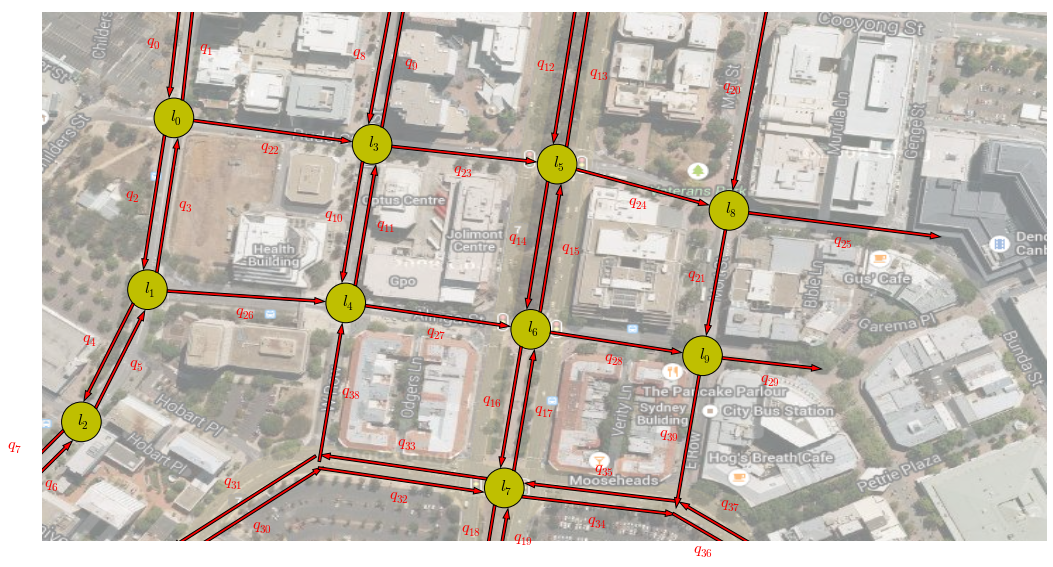
\includegraphics[width=0.7\textwidth,trim={1cm 1cm 0cm 1cm},clip]{map_overlay.png}
}
\subfigure[]{
\label{subfig:converg_a}
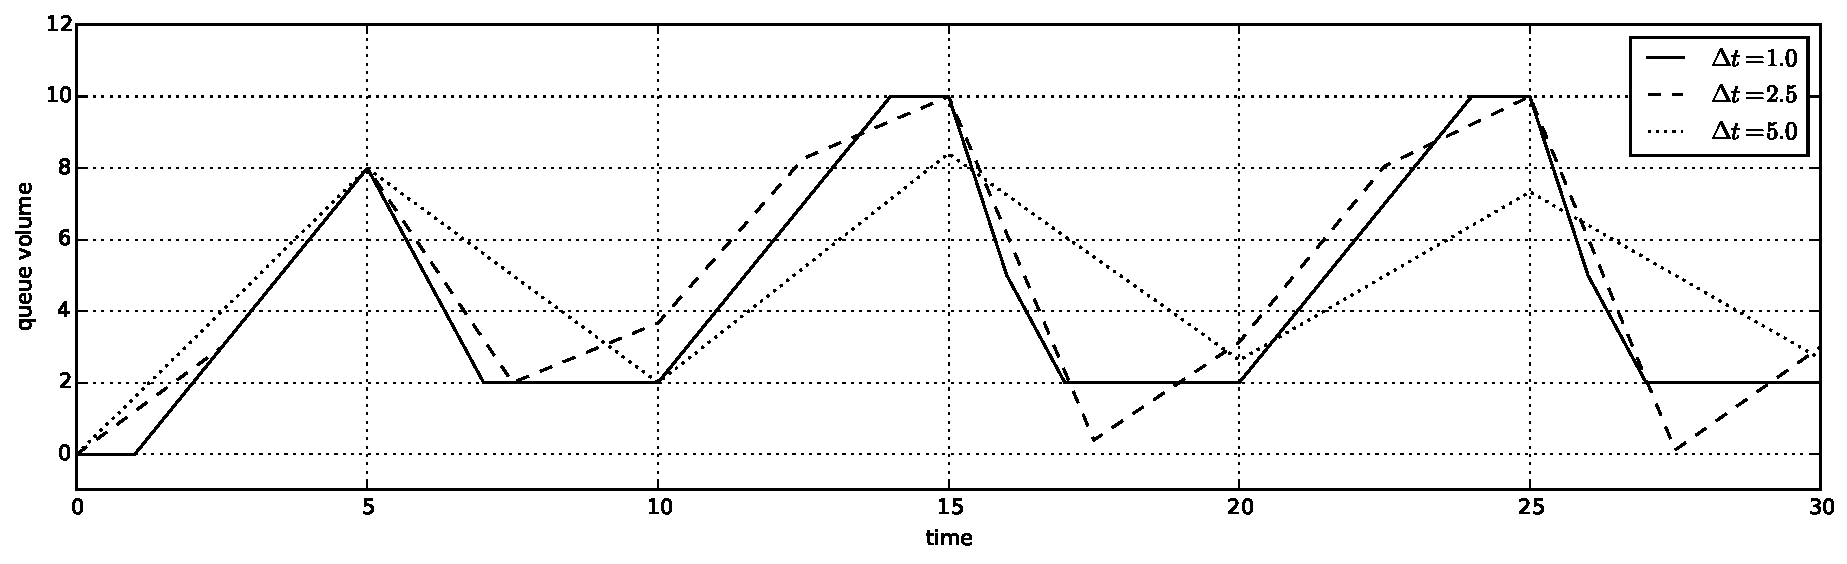
\includegraphics[width=1.0\textwidth,trim={0cm 0cm 0cm 0cm},clip]{convergence.pdf}
}
\subfigure[]{
\label{subfig:converg_b}
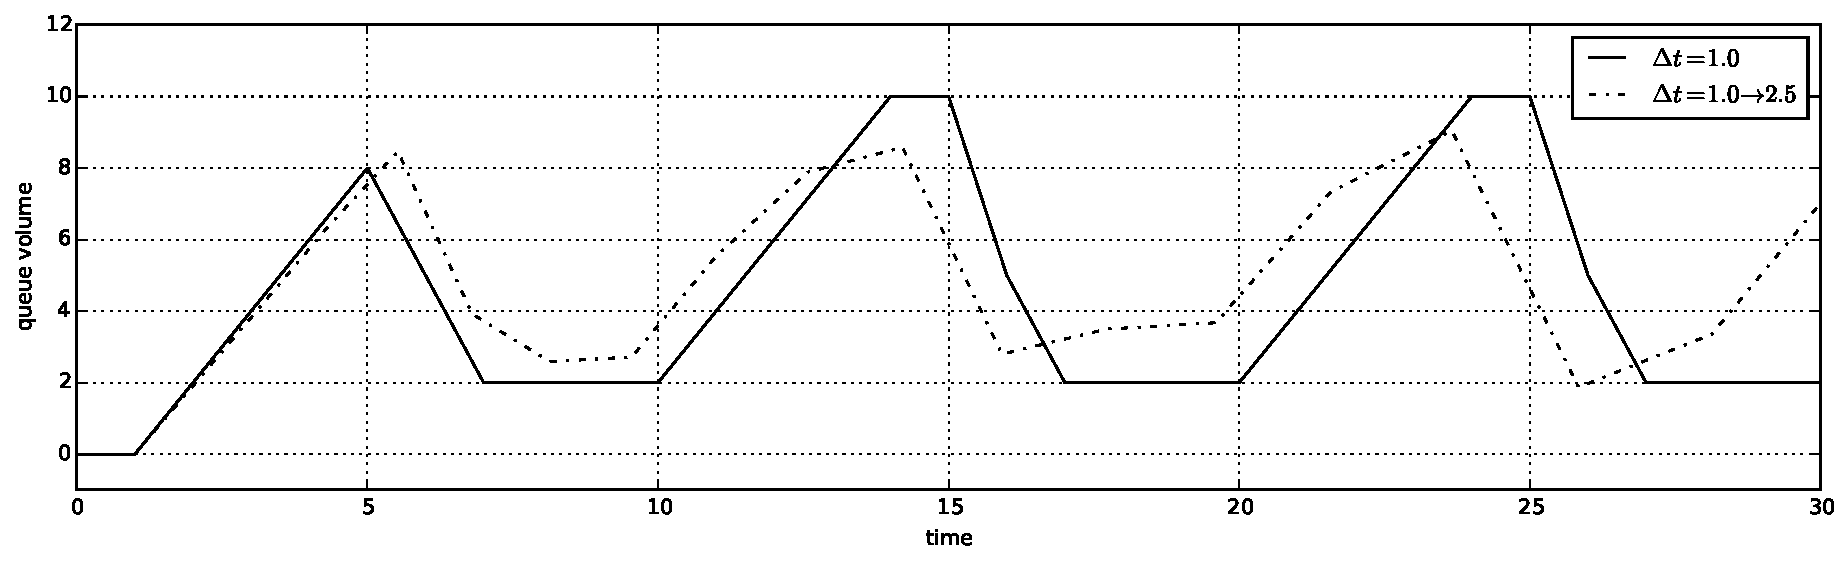
\includegraphics[width=1.0\textwidth,trim={0cm 0cm 0cm 0cm},clip]{convergence_vari.pdf}
}
\caption{A QTM example showing the evolution of traffic volume in $q_{27}$ over
time. (a) Streetmap overlay showing how each queue in QTM network corresponds to a segment of roadway and each light to a controlled intersection. (b) Convergce with increasing refinement of $\Delta t$ from $5.0$ down to
$1.0$. (c) Dilation of $\Delta t$ from $1.0$ to $2.5$ compared to a fixed
$\Delta t$ of $1.0$.}

\end{figure*}

\begin{figure*}[t!]
\centering
%  trim={<left> <lower> <right> <upper>}
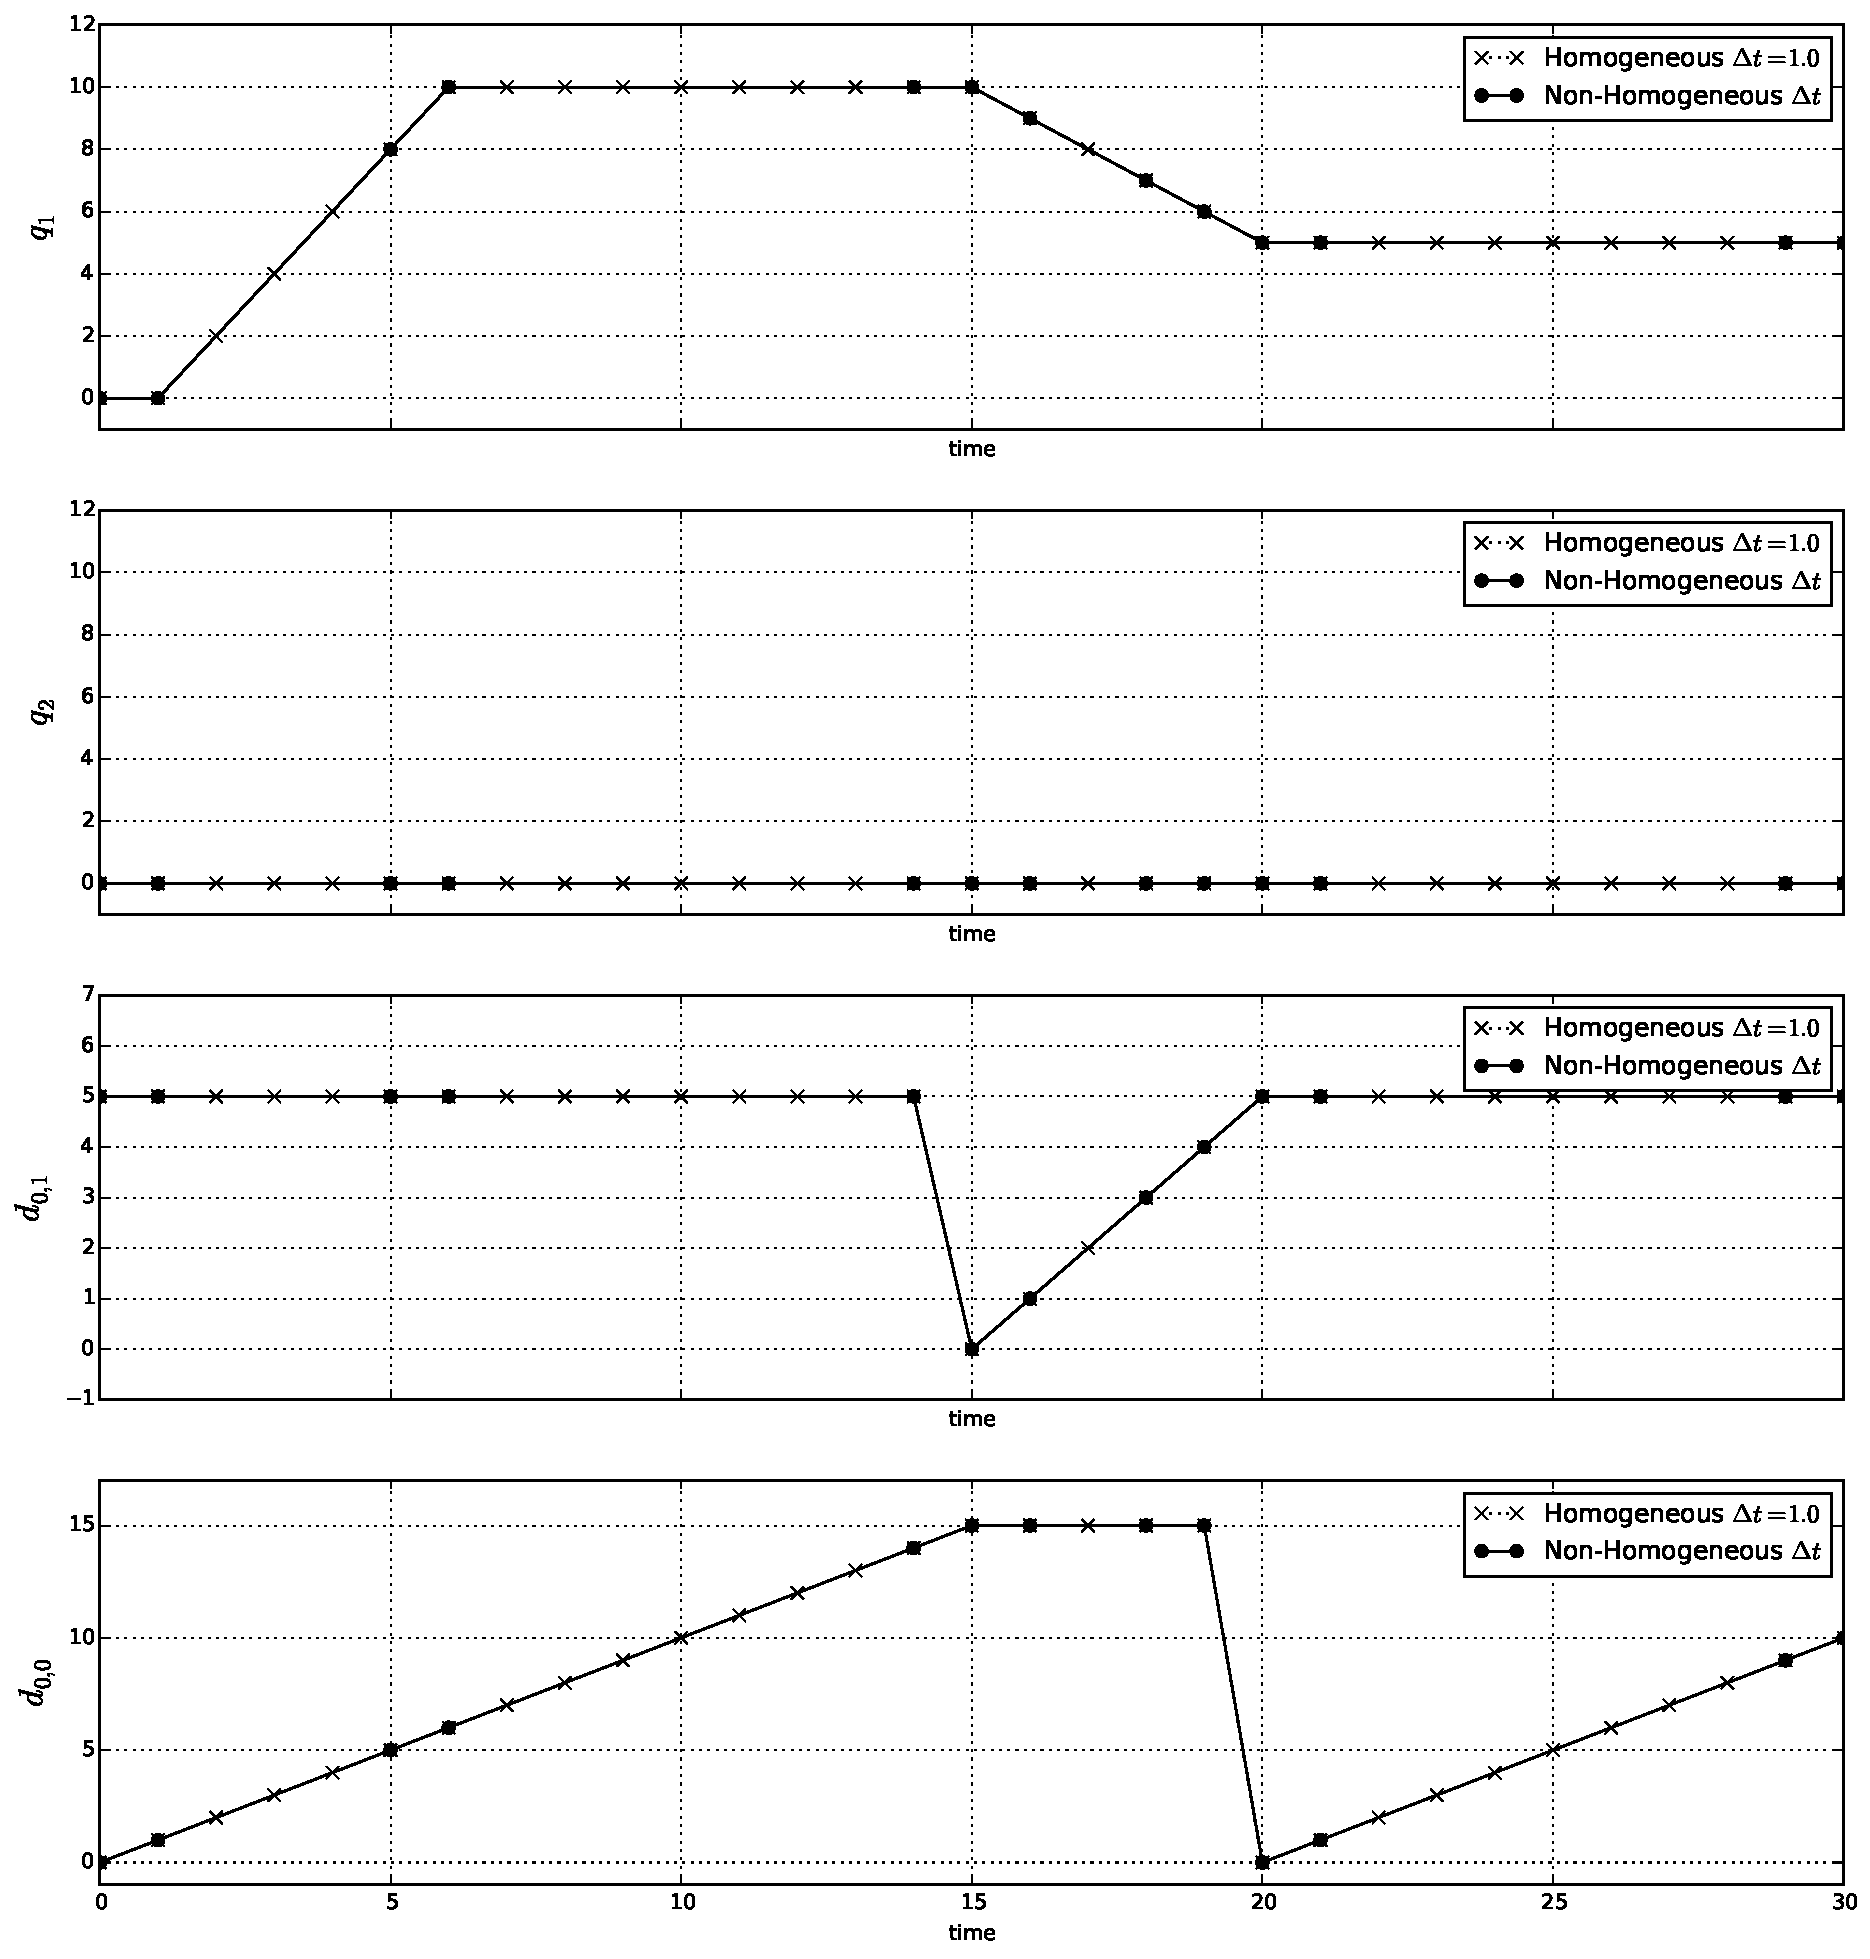
\includegraphics[width=1.0\textwidth,trim={0cm 0cm 0cm 0cm},clip]{convergence_NH.pdf}
\caption{An example showing the convergence between a homogeneous solution with
$\Delta t=1.0$ and a non-homogeneous solution over 30 seconds for the same
network. By using non-homogeneous time steps the same solution is found with
only 14 sample points compared to 30 for homogeneous solution.}
\label{fig:converg_c}
\end{figure*}



As with MILP formulations of CTM (e.g. \trbcite{lin2004enhanced}),
QTM is also susceptible to \emph{withholding traffic}, i.e., the
optimizer might prevent cars from moving from $i$ to $j$ even though the
associated traffic phase is active and $j$ is not full.
%
We address this issue through our objective function~\eqref{eq:objFunc} by
maximizing the total outflow~\qout{i}~(i.e., both internal and external outflow)
of~$i$ plus the inflow~\inq{i} from the outside of the network to~$i$.
%
This quantity is weighted by the remaining time until the end of the simulation
horizon \TMAX to force the optimizer to allow as much traffic volume as possible
into the network and move traffic to the outside the network as soon as
possible.
%
\eqref{eq:objFunc} is analogous to minimizing delay in CTM models,
e.g., \eqref{eq:objFunc} is equivalent to the objective function (O3) in
\trbcite{lin2004enhanced} for their parameters $\alpha = \beta = 1$. \toIain{Add
a paragraph linking the plots with the objective function.}
\fnremark{Show diagrams with traffic predictions converging as time increment gets
smaller.  Validates that large time-steps are rough approximations while model
behavior converges for small time steps.}
%% FWT: not sure if we need to give this extra details
%\trbcite{lin2004enhanced} derive an objective function for the minimisation of
%total delay based on the difference between the cumulative departure and
%arrival curves at the origin and destination. However, such an approach
%requires the network to be cleared at the end of the optimisation period.


\begin{equation}
\max 
 \sum_{n=1}^{\Nn} \sum_{i=1}^{\Qn} (\TMAX - \tn + 1) (\qout{i} + \inq{i})
\tag{O1}\label{eq:objFunc}
\end{equation}


The objective function~\eqref{eq:objFunc} and
constraints~(\ref{c:turnProb}--\ref{c:10}) form the LP representing the
dynamic, piecewise linear model of flow in a QTM network over time when a
control plan \p{\tl}{k} is given as an input parameter.

\cref{subfig:converg_a,subfig:converg_b,fig:converg_c} show the results of applying the LP formulation to a simple model with a fixed signal plan, using both homogeneous \vecDT and non-homogeneous \vecDT.



\section{Traffic Control with QTM as an MILP}\label{sec:milp}

In this section, we remove the assumption that a valid control plan for all
traffic lights is given and extend the LP
(\ref{eq:objFunc},~\ref{c:turnProb}--\ref{c:10}) to an Mixed-Integer LP (MILP)
that also computes the optimal control plan.
%
Formally, for all~$\tl \in \Lset$, $k \in \Pset_\tl$, and interval $n \in
\{1,\dots,N\}$, the phase activation parameter~$\p{\tl}{k} \in \{0,1\}$ becomes
a free variable to be optimized.
%
In order to obtain a valid control plan, we enforce that one phase of traffic
light \tl is always active at any interval~$n$~\eqref{c:onlyOnePhaseOn} and that
phase changes happen sequentially~\eqref{c:seqPhases}, i.e., if phase~$k$ was
active during interval~$n-1$ and has become inactive in interval~$n$, then
phase~$k+1$ must be active in interval~$n$.
%
\eqref{c:seqPhases} assumes that $k+1$ equals 1 if $k = \Pn{}$.
%
\toIain{I removed the constraint $\p{\ell}{k} + \p{\ell}{k+1} \le 1$ because it
is subsumed by $\p{\ell}{k} \in \{0,1\}$ and \eqref{c:onlyOnePhaseOn}}


%% FWT: note sure if the text bellow is necessary
%Note that there could be more than one queue mapped to each $\p[]{\ell}{k}$, or
%their could be none

\begin{cAlign}
%
\sum\limits_{k=1}^{\Pn} \p{\ell}{k} &= 1\tagconstrain{c:onlyOnePhaseOn}\\
%
\p[n-1]{\ell}{k} &\le \p{\ell}{k} + \p{\ell}{k+1}\tagconstrain{c:seqPhases}
%
\end{cAlign}


Next, we enforce the minimum and maximum phase durations (i.e.,
$\PTMIN{\ell}{k}$ and $\PTMAX{\ell}{k}$) for each phase $k \in \Pset_\tl$ of
traffic light \tl.
%
To encode these constraints, we use the helper variable $\pd{\ell}{k} \in
[0,\PTMAX{\ell}{k}]$ defined by constraints (\ref{c:pd:incUB}--\ref{c:pd:reset})
that:
%
(i) holds the elapsed time since the start of phase $k$ when $\p[n]{\ell}{k}$ is
active~(\ref{c:pd:incUB},\ref{c:pd:incLB}) (\cref{subfig:test1});
%
(ii) is constant and holds the duration of the last phase until the next
activation when $\p[n]{\ell}{k}$ is
inactive~(\ref{c:pd:inactiveUB},\ref{c:pd:inactiveLB}) (\cref{subfig:test2}); and
%
(iii) is restarted when phase~$k$ changes from inactive to
active~\eqref{c:pd:reset} (\cref{subfig:test3}).
%
Notice that (\ref{c:pd:incUB}--\ref{c:pd:reset}) employs the \textit{big-M}
method to turn the cases that should not be active into subsumed constraints
based on the value of $\p[]{\tl}{k}$.
%
We use~\PTMAX{\ell}{k} as our large constant since $\pd[n]{\ell}{k} \le
\PTMAX{\ell}{k}$ and $\DT[n] \le \PTMAX{\ell}{k}$ by assumption (\cref{sec:lp}).
%
Similarly, \cref{c:minPhase} ensures the minimum phase time of $k$ and is
not enforced while $k$ is still active.
%
%% FWT: I think the mathematical definition of \pd is redundant now.
%\begin{equation}
%\pd{\ell}{k} = 
%\begin{cases}
%\pd[n-1]{\ell}{k} + \DT[n-1] & \p[n-1]{\ell}{k}=1,\p{\ell}{k}=1\\
%\pd[n-1]{\ell}{k} & \p{\ell}{k}=0\\
%0 & \p[n-1]{\ell}{k}=0,\p{\ell}{k}=1
%\end{cases}
%\label{def:pd}
%\end{equation}
%
%% TODO(fwt): I believe that that \pd{\ell}{k} (above) could be redefined by
%% shifting it by delta_n resulting in a d_{l,k,n} representing the total time
%% until the end of interval **n** instead of n-1. This would be more intuitive
%% and would simplify c:cycleLB and c:cycleUB. This is what I propose:
%% d_{l,k,n} = d_{l,k,n-1} + delta-t_{n}  if p_{l,k,n-1} = p_{l,k,n} = 1
%%           = d_{l,k,n-1}                if p_{l,k,n} = 0
%%           = delta-t_{n}                if p_{l,k,n-1} 0 and p_{l,k,n} = 1
%
%% FWT: this constraint is define as the variable domain
%\pd{\ell}{k} &\le \PTMAX{\ell}{k}\tag{C19}\label{eq:C19}\\
%
\begin{cAlign}
%
\pd{\ell}{k} &\le
  \pd[n-1]{\ell}{k} + \DT[n-1] \p[n-1]{\ell}{k} 
  + \PTMAX{\ell}{k} (1 - \p[n-1]{\ell}{k})\tagconstrain{c:pd:incUB}\\
%
\pd{\ell}{k} &\ge
  \pd[n-1]{\ell}{k} + \DT[n-1] \p[n-1]{\ell}{k}
  - \PTMAX{\ell}{k} (1 - \p[n-1]{\ell}{k})\tagconstrain{c:pd:incLB}\\
%
\pd{\ell}{k} &\le \pd[n-1]{\ell}{k} + \PTMAX{\ell}{k} \p[n-1]{\ell}{k}
  \tagconstrain{c:pd:inactiveUB} \fnremark{check the n-1 in \eqref{c:pd:inactiveUB}}\\ 
%
\pd{\ell}{k} &\ge \pd[n-1]{\ell}{k} - \PTMAX{\ell}{k} \p{\ell}{k}
  \tagconstrain{c:pd:inactiveLB}\\
%
\pd{\ell}{k} &\le \PTMAX{\ell}{k}(1 - \p{\ell}{k} + \p[n-1]{\ell}{k})
  \tagconstrain{c:pd:reset}\\
%
\pd{\ell}{k} &\ge \PTMIN{\ell}{k}(1 - \p{\ell}{k}) \tagconstrain{c:minPhase}
\end{cAlign}



Finally, we constrain the sum of all the phase durations for light \tl to be
within the cycle time limits \CTMIN{\tl}~\eqref{c:cycleLB} and
\CTMAX{\tl}~\eqref{c:cycleUB} (\cref{subfig:test4}).
%
In both \eqref{c:cycleLB} and \eqref{c:cycleUB}, we use the duration of phase 1
of \tl from the previous interval $n-1$ instead of the current interval $n$
because \eqref{c:pd:reset} forces \pd[n]{\tl}{1} to be 0 at the beginning of
each cycle;
%
however, from the previous end of phase 1 until $n-1$, \pd[n-1]{\tl}{1} holds
the correct elapse time of phase 1.
%
Additionally, \eqref{c:cycleLB} is enforced right after the end of the each
cycle, i.e., when its first phase is changed from inactive to active.
%
\toIain{Relate the phase and cycle constraints with the plots}
%
\begin{cAlign}
%
\pd[n-1]{\ell}{1} + \sum\limits_{k=2}^{\Pn} \pd{\ell}{k} &\ge \CTMIN{\ell}
(\p{k}{1} - \p[n-1]{k}{1}) \tagconstrain{c:cycleLB}\\
%
\pd[n-1]{\ell}{1} + \sum\limits_{k=2}^{\Pn} \pd{\ell}{k} &\le \CTMAX{\ell}
\tagconstrain{c:cycleUB}
%
\end{cAlign}
The MILP that encodes the problem of finding the optimal traffic control plan in
a QTM network is defined
by~(\ref{eq:objFunc},~\ref{c:turnProb}--\ref{c:cycleUB}).
%\fnremark{Extend the conclusion of this section}


\begin{figure*}[t!]
\centering
%  trim={<left> <lower> <right> <upper>}
\subfigure[]{
\label{subfig:test1}
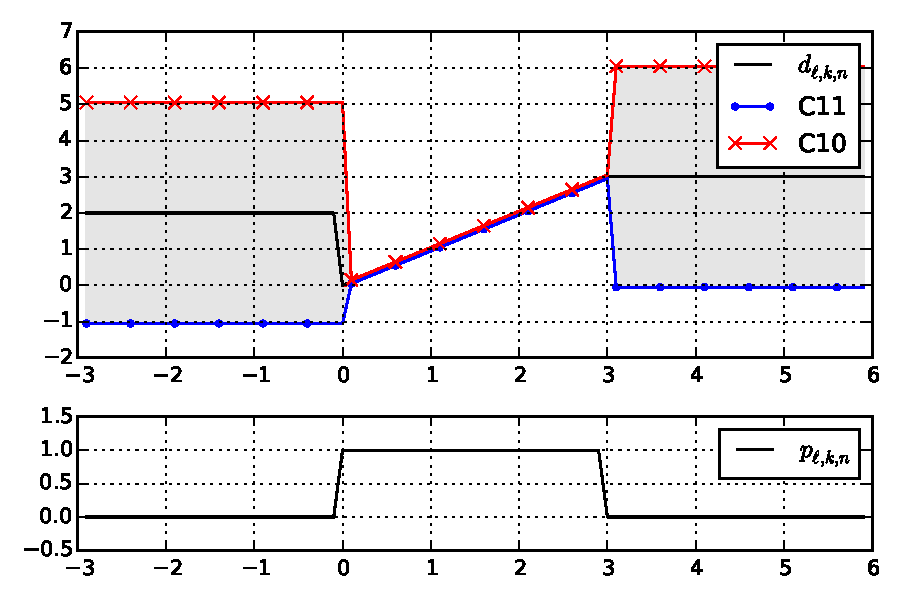
\includegraphics[width=0.45\textwidth,trim={0cm 0cm 0cm 0cm},clip]{phase_plot_fig_1.pdf}}
\subfigure[]{
\label{subfig:test2}
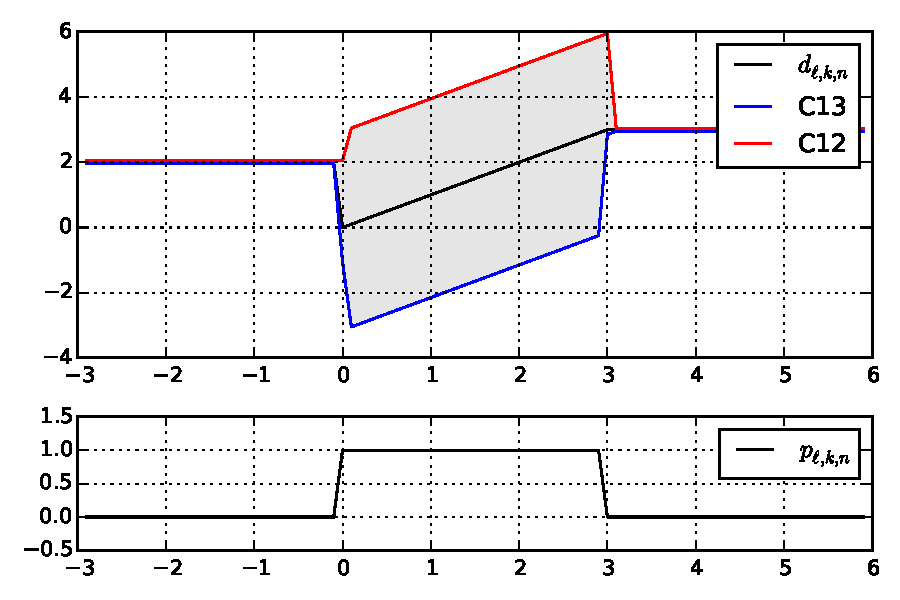
\includegraphics[width=0.45\textwidth,trim={0cm 0cm 0cm 0cm},clip]{phase_plot_fig_2.pdf}}
\subfigure[]{
\label{subfig:test3}
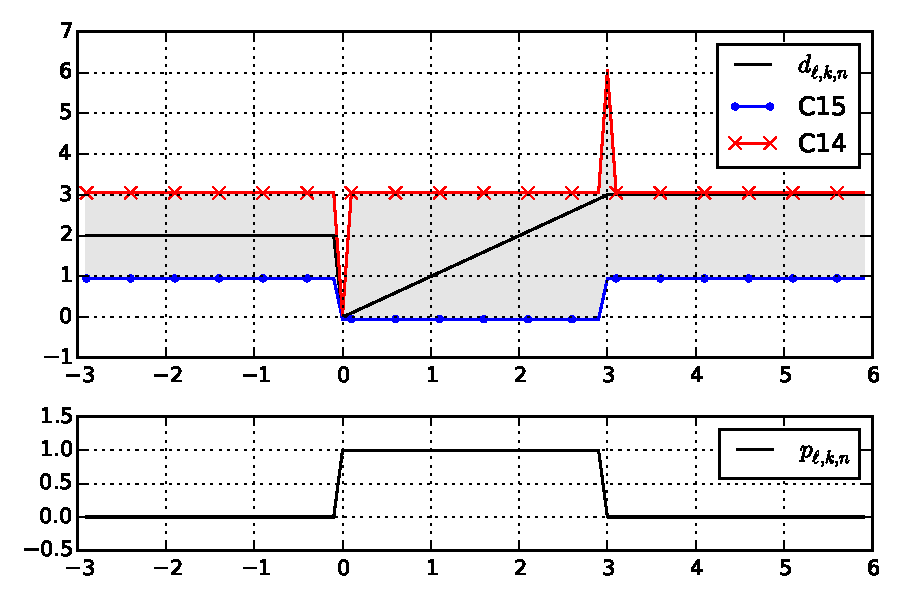
\includegraphics[width=0.45\textwidth,trim={0cm 0cm 0cm 0cm},clip]{phase_plot_fig_3.pdf}}
\subfigure[]{
\label{subfig:test4}
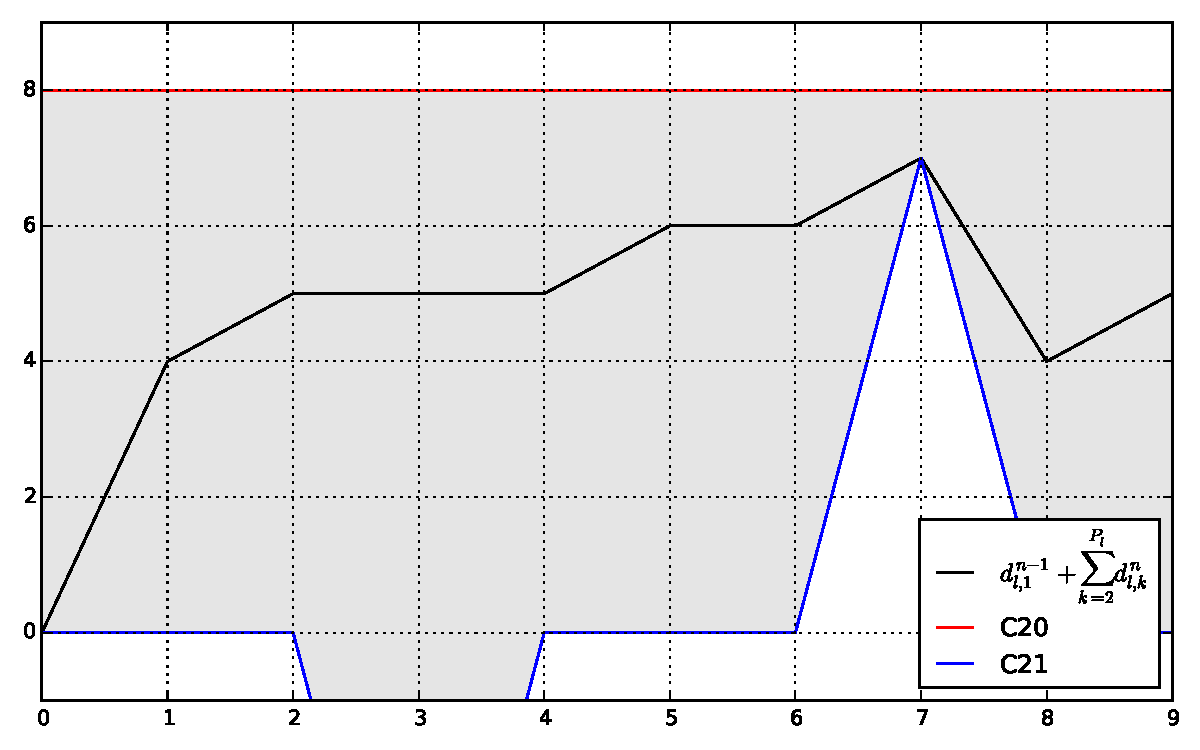
\includegraphics[width=0.45\textwidth,trim={0cm 0cm 0cm 0cm},clip]{phase_plot_fig_4.pdf}}
\caption{An example showing the phase and cycle time constraint envelopes. In
(a), (b) and (c), $\PTMIN{\ell}{k}=1$ and $\PTMAX{\ell}{k}=3$, the duration of
the previous activation was 2 and the duration of the current activation is 3.
In (d), the total cycle time is 7 with $\CTMIN{\ell}=7$, $\CTMAX{\ell}=8$}
\label{fig:phase_plots}
\end{figure*}



\section{Empirical Evaluation}
  
In this section we compare the solutions for traffic networks modeled as a QTM
using homogeneous and non-homogeneous time intervals w.r.t.\ to two evaluation criteria:
%
the quality of the solution and convergence to the optimal solution vs.\ the number
of time steps.
%
% TODO \fnremark{FWT: I don't think that optimal is the best word here since
%we arbitrarily fixed a value of \DT[]. Also, there is the technical problem that
%Gurobi might not have found the true optimal.}
%
Specifically, we compare the quality of solutions based on the total travel time and we also
consider the third quartile and maximum of the observed delay distribution.
%
%% TODO(fwt): maybe define what we mean by optimal here, for instance
%
%For our experiments, we consider as optimal solution, the MILP solution of a
%QTM using small enough homogeneous \DT[] with unlimited computational
%resources.
%
Our hypotheses are:
%
(i) the quality of the non-homogeneous solutions is at least as good as the
homogeneous ones when the number of time intervals~\Nn is fixed; and 
%
(ii) the non-homogeneous approach requires less time intervals (i.e., smaller
\Nn) than the homogeneous approach to converge to the optimal solution.
%
In the remainder of this section, we present the traffic networks considered in
the experiments, our methodology, and the results.



\subsection{Networks}



\begin{figure*}[t!]
\centering
%  trim={<left> <lower> <right> <upper>}
\subfigure[]{
\label{subfig:network1}
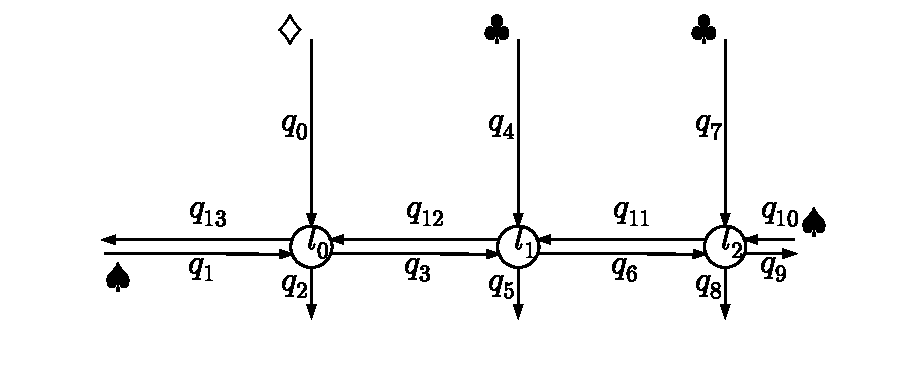
\includegraphics[width=0.45\textwidth]{network_1.pdf}}
\subfigure[]{
\label{subfig:network2}
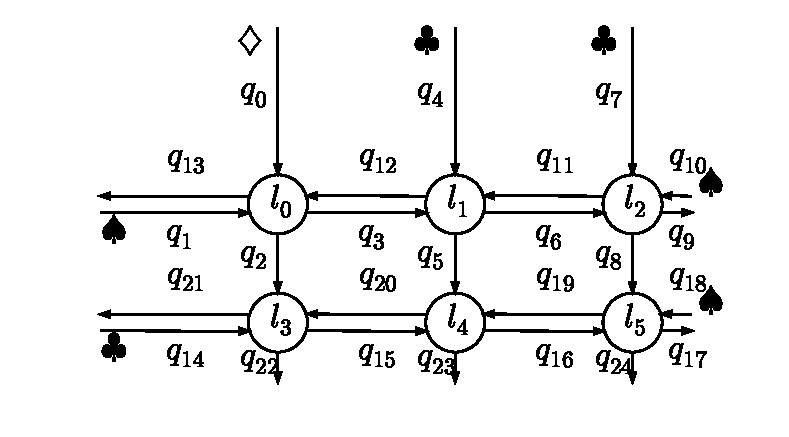
\includegraphics[width=0.45\textwidth]{network_2.pdf}}
\subfigure[]{
\label{subfig:network3}
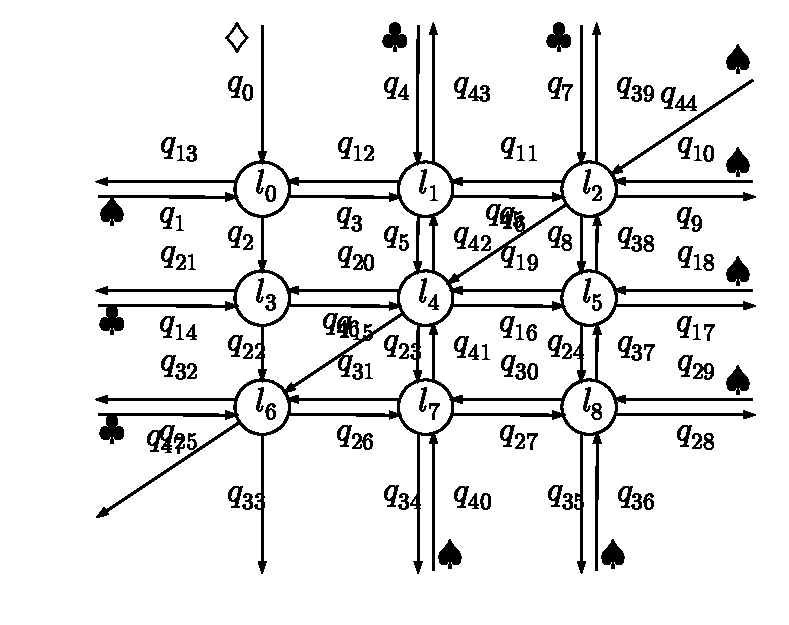
\includegraphics[width=0.45\textwidth]{network_3.pdf}}
\subfigure[]{
\label{subfig:demand_plot}
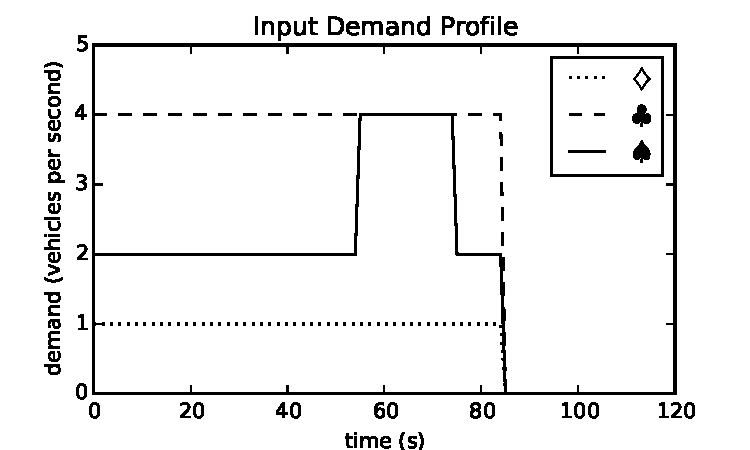
\includegraphics[width=0.45\textwidth]{demand_plot.pdf}}
\caption{(a--c) Networks used to evaluate the QTM performance.
%
(d) Demand profile of the queues marked as \qLowTraf,
\qHighTraf, and \qVarTraf for our experiments.}
\label{fig:networks}
\end{figure*}



We consider three networks of increasing complexity (\cref{fig:networks}): an
avenue crossed by three side streets; a 2-by-3 grid; and a 3-by-3 grid with a
diagonal avenue.
%
The queues receiving cars from outside of the network are marked in
\cref{fig:networks} and we refer to them as input queues.
%
The maximum queue capacity~(\QMAX{i}) is 60 cars for non-input queues and
infinity for input queues to prevent interruption of the input demand due to
spill back from the stop line. 
%
The traversal time of each queue $i$~(\QDELAY{i}) is set at 9s (a distance of
about 100m with a free flow speed of 50km/h).
%
Flows are defined from the head of each queue $i$ into the tail of the next
queue $j$;
%
there is no turning traffic ($\FTURN{i}{j}=1$), and the maximum flow rate
between queues, \FMAX{i}{j}, is set at 5 cars/s.
%
All traffic lights have two phases, north-south and east-west, and lights 2, 4
and 6 of network 3 have the additional northeast-southwest phase to control the
diagonal avenue.
%
For networks 1 and 2, \PTMIN{\tl}{k} is 1s, \PTMAX{\tl}{k} is 3s, \CTMIN{\tl} is
2s, and \CTMAX{\tl} is 6s, for all traffic light \tl and phase $k$.
%
For network 3, \PTMIN{\tl}{k} is 1s and \PTMAX{\tl}{k} is 6s for all \tl and
$k$; and \CTMIN{\tl} is 2s and \CTMAX{\tl} is 12s for all lights \tl except for
lights 2, 4 and 6 (i.e., lights also used by the diagonal avenue) in which
\CTMIN{\tl} is 3s and \CTMAX{\tl} is 18s.




\subsection{Experimental Methodology}

%\begin{table}[h]
%\caption{Network Demand Profiles (vehicles per second)}
%\label{tab:network_demand}
%\centering
%\begin{tabular}{cccccc}
%\toprule
%& Inflow Queues & 0 - 55 s & 55 - 70 s & 70 - 85 s & > 85 s\\
%\midrule
%\multirow{2}{*}{Network 1}&$q_0$ & 1 & 1 & 1 & 0 \\
%&$q_4, q_7$ & 4 & 4 & 4 & 0 \\
%&$q_1,q_{10}$& 2 & 4 & 2 & 0 \\
%\midrule
%\multirow{2}{*}{Network 2}&$q_0$ & 1 & 1 & 1 & 0 \\
%&$q_4,q_7,q_{14}$& 4 & 4 & 4 & 0 \\
%&$q_1, q_{10},q_{18}$ & 2 & 4 & 2 & 0 \\
%\midrule
%\multirow{2}{*}{Network 3}&$q_0$ & 1 & 1 & 1 & 0 \\
%&$q_4,q_7,q_{14},q_{25},$& 4 & 4 & 4 & 0 \\
%&$q_1, q_{10},q_{18},q_{29},q_{36},q_{40},q_{44}$ & 2 & 4 & 2 & 0 \\
%\bottomrule\\
%\end{tabular}
%\end{table}


For each network, a constant background level traffic is injected in the network
in the first 55s to allow the solver to settle on a stable policy.
%
Then a spike in demand is introduced in the queues marked as \qVarTraf
(\cref{fig:networks}) from time 55s to 70s to trigger a policy change.
%
%with the expectation that plans generated with longer look ahead will produce a
%more coordinated global policy change.
%
From time 70s to 85s, the demand is returned to the background level, and then
reduced to zero for all input queues.
%
We extend the problem horizon~\TMAX until all cars have left the network.
%
By clearing the network, we can easily measure the total travel time for all the
traffic as the area between the cumulative arrival and departure curves measured
at the boundaries of the network.
%
%TODO \fnremark{FWT: is this explanation of how to compute the total travel time
%still necessary?}
%
%\cref{tab:network_demand} presents the demand profile of each network.
%
The background level for the input queues are 1, 4 and 2 cars/s for queues
marked as \qLowTraf, \qHighTraf and \qVarTraf (\cref{subfig:demand_plot}),
respectively; and during the high demand period, the queues \qVarTraf receive 4
cars/s.




\begin{figure*}[t!]
\centering
%  trim={<left> <lower> <right> <upper>}
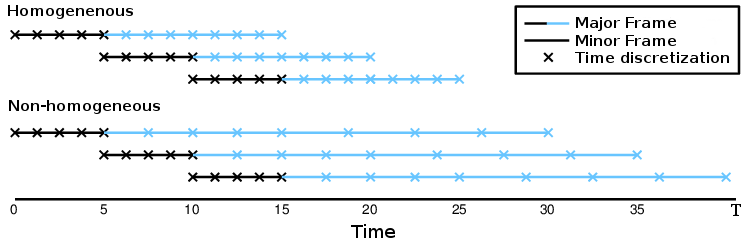
\includegraphics[width=0.75\textwidth]{non_homogeneous_control.png}
\caption{Receding horizon control. In this example, the problem
  horizon \TMAX is 40s. The major frames for MILP optimization are
  discretized in 12 time intervals ($\Nn = 12$) and they span 15s and
  30s for homogeneous and non-homogeneous discretizations,
  respectively.  The minor frames represent the prefix of the 
  major frame MILP optimization that is executed.  The horizon
  recedes by the minor frame duration after each execution.}
\label{fig:multiplan}
\end{figure*}


% def major and minor frame tell about overlapping and fig:multiplan show
% parameters, i.e., delta ts
% - fairness: same delta t for minor frame
For both homogeneous and non-homogeneous intervals, we use the MILP QTM
formulation~(\cref{sec:milp}) in a receding horizon manner: a control plan is
computed for a pre-defined horizon (smaller than \TMAX) and only a prefix of
this plan is executed before generating a new control plan. 
%
\cref{fig:multiplan} depicts our receding horizon approach and we refer to the
planning horizon as a major frame and its executable prefix as a minor frame.
%
Notice that, while the plan for a minor frame is being executed, we can start
computing the solution for the next major frame based on a forecast model.


To perform a fair comparison between the homogeneous and non-homogeneous
discretizations, we fix the size of all minor frames to 10s and force it to be
discretized in homogeneous intervals of 0.25s.
%
For the homogeneous experiments, \DT[] is kept at 0.25s throughout the major
frame; therefore, given \Nn, the major frame size equals $\Nn/4$ seconds for the
homogeneous approach.
%
For the non-homogeneous experiments, \DT[] linearly increases from
0.25s at the end of the minor frame to 1.0s at the end of the major frame;
therefore, the major frame size used by the non-homogeneous approach
is $10.375 + 0.625(\Nn-40)$ seconds for a given $\Nn > 40$.
%
%We analyze the effect of the major frame size by varying it from 20s through to 
%120s.
%
% explain evaluation: concatenation + LP simulation Overall ``optimal'' for
% comparison
Once we have generated a series of minor frames, we concatenate them into a
single plan and simulate the flow through the network using the QTM LP
formulation with a fixed (homogeneous) $\DT[]$ of 0.25s.
%
%TODO \fnremark{Do we need to justify why we use the QTM as the simulator over
%say a micro simulator?}
%
We also compare both receding horizon approaches against the optimal solution
obtained by computing a single control plan for the entire control horizon
(i.e., $[0,\TMAX]$) using a fixed \DT[] of 0.25s.


For all our experiments, we used Gurobi\textsuperscript{TM} as the MILP solver with
12 threads on a 3.1GHz AMD Opteron\textsuperscript{TM}~4334 processor with 12
cores.
%
We limit the MIP gap accuracy to 0.1\% and the time cutoff for solving a major
frame to 3000s for the receding horizon approaches and unbounded in order to
determine the optimal minimum travel time solution to which all other solutions are compared.
%
%% \toIain{Can you explain the following better and provide evidence:
%% \textit{while we can solve non-homogeneous major frames up to convergence in
%% real time, we extend the solve time limit to 3000s for all test points for a
%% fair comparison with the homogeneous test points.}?
%%
%% Iain: Deleted as it was not strictly true. Either we re-run scaled up on AWS
%% with 10s solver time limit. Or we perhaps explain that 3000s shows that it
%% could be scaled up to real time}
%
All our results are averaged over five runs to account for Gubori's
stochastic strategies.



%\begin{table}[h]
%\caption{Network 3 traffic parameters}
%\label{tab:net3wave}
%\centering
%\begin{tabular}{cccccc}
%\toprule
%Queue & Background & End & Wave & Start &End\\ 
%\midrule
%$q_0$ & 1 & 85 & 1 & 55 & 70\\
%$q_1$ & 2 & 85 & 4 & 55 & 70\\
%$q_4$ & 4 & 85 & 4 & 55 & 70\\
%$q_7$ & 4 & 85 & 4 & 55 & 70\\
%$q_{10}$ & 2 & 85 & 4 & 55 & 70\\
%$q_{14}$ & 4 & 85 & 4 & 55 & 70\\
%$q_{18}$ & 2 & 85 & 4 & 55 & 70\\
%$q_{25}$ & 4 & 85 & 4 & 55 & 70\\
%$q_{29}$ & 2 & 85 & 4 & 55 & 70\\
%$q_{36}$ & 2 & 85 & 4 & 55 & 70\\
%$q_{40}$ & 2 & 85 & 4 & 55 & 70\\
%$q_{44}$ & 2 & 85 & 4 & 55 & 70\\
%\bottomrule\\
%\end{tabular}
%\end{table}


\subsection{Results}


\begin{figure*}[t!]
\centering
%  trim={<left> <lower> <right> <upper>}
\subfigure[]{
\label{subfig:travel_time_3}
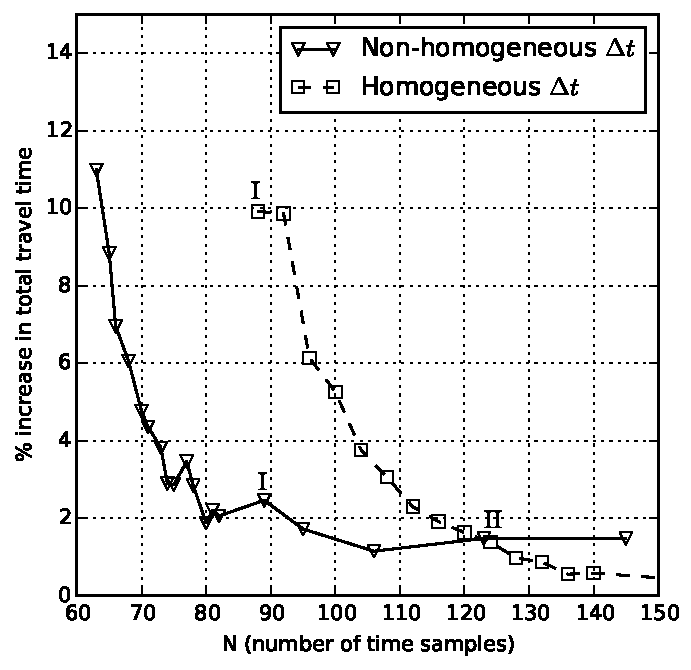
\includegraphics[keepaspectratio,height=0.3225\textwidth]{network_1_converge.pdf}}
\subfigure[]{
\label{subfig:delay_3}
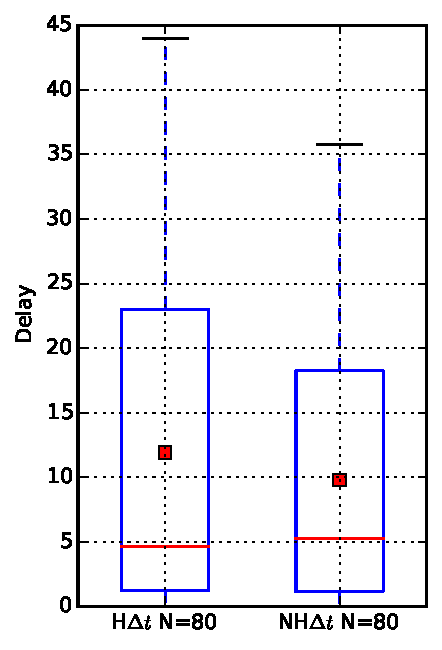
\includegraphics[keepaspectratio,height=0.3225\textwidth]{box_plot_early_3l.pdf}
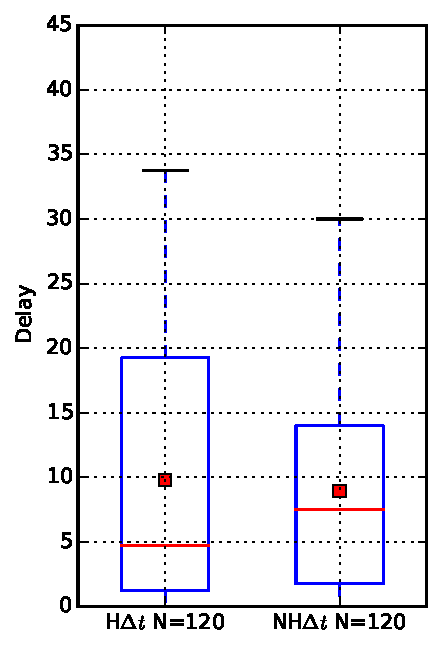
\includegraphics[keepaspectratio,height=0.3225\textwidth]
{box_plot_converg_3l.pdf}
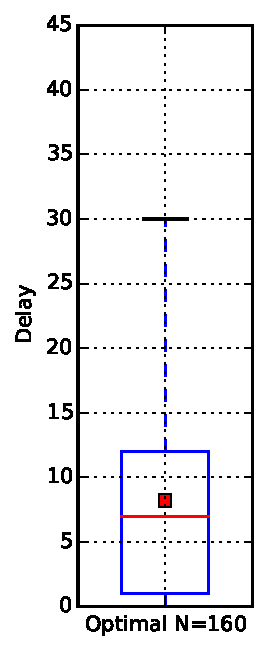
\includegraphics[keepaspectratio,height=0.3225\textwidth]{box_plot_final_3l.pdf}}

\subfigure[]{
\label{subfig:travel_time_6}
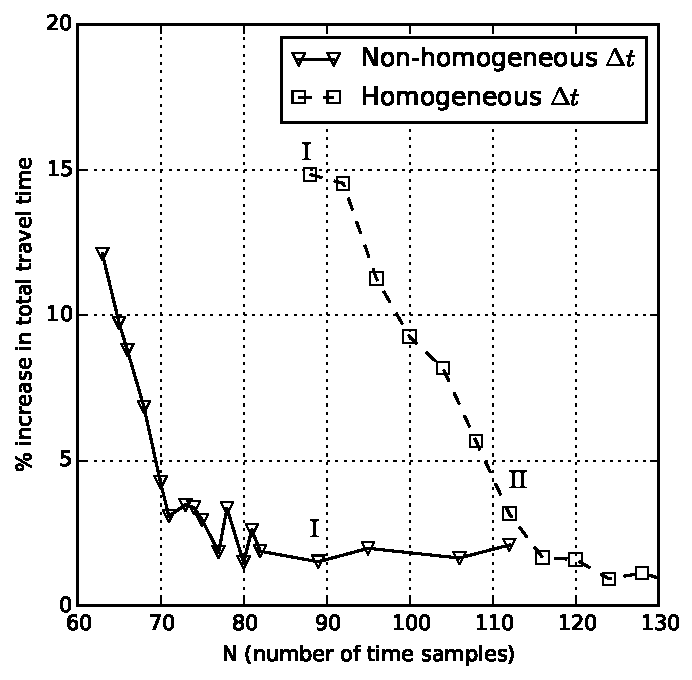
\includegraphics[keepaspectratio,height=0.3225\textwidth]{network_2_converge.pdf}}
\subfigure[]{
\label{subfig:delay_6}
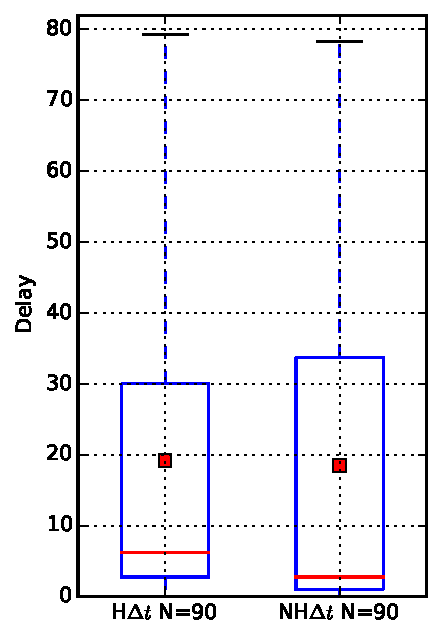
\includegraphics[keepaspectratio,height=0.3225\textwidth]{box_plot_early_6l.pdf}
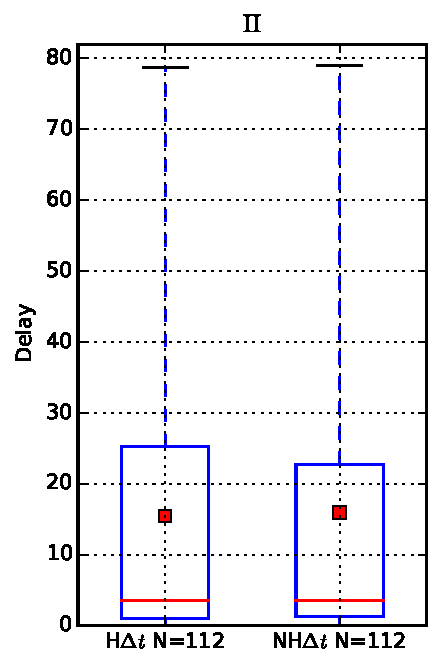
\includegraphics[keepaspectratio,height=0.3225\textwidth]
{box_plot_converg_6l.pdf}
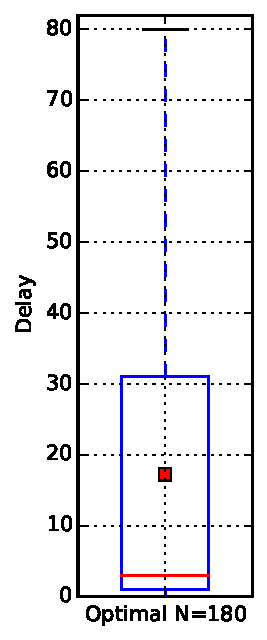
\includegraphics[keepaspectratio,height=0.3225\textwidth]{box_plot_final_6l.pdf}}

\subfigure[]{
\label{subfig:travel_time_9}
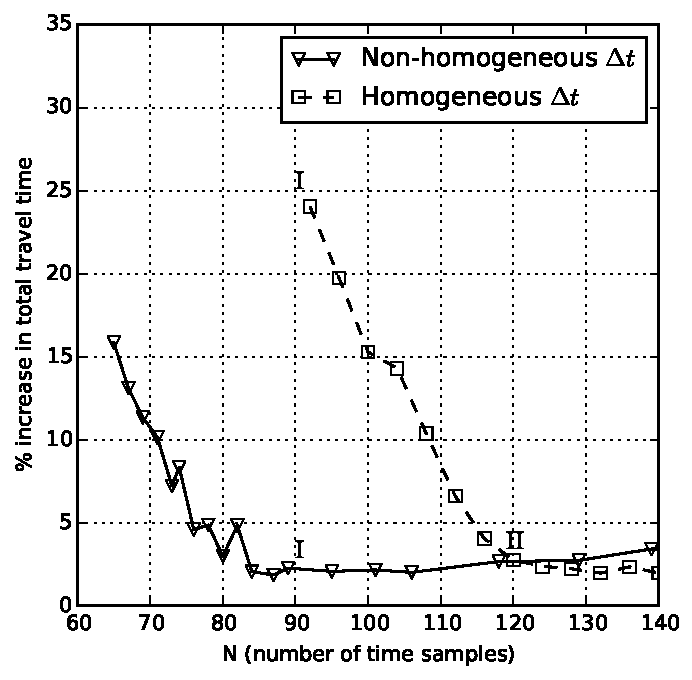
\includegraphics[keepaspectratio,height=0.3225\textwidth]{network_3_converge.pdf}}
\subfigure[]{
\label{subfig:delay_9}
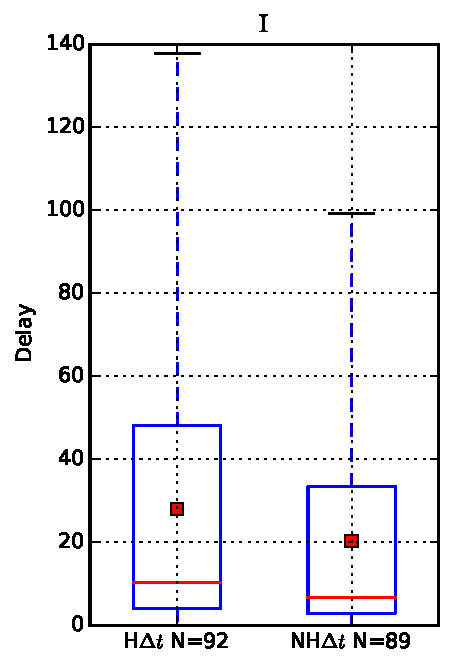
\includegraphics[keepaspectratio,height=0.3225\textwidth]{box_plot_early_9l.pdf}
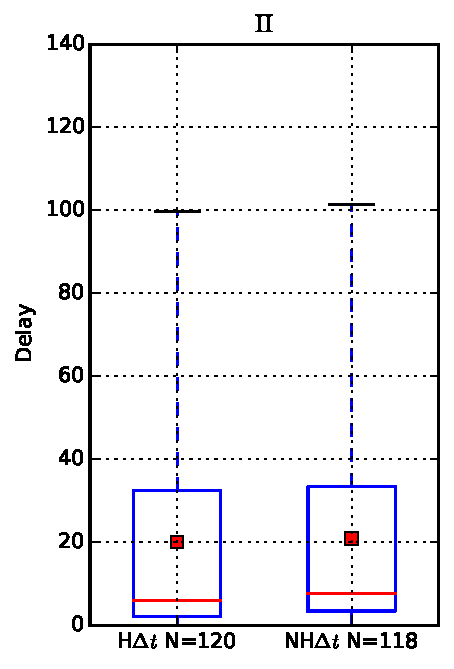
\includegraphics[keepaspectratio,height=0.3225\textwidth]
{box_plot_converg_9l.pdf}
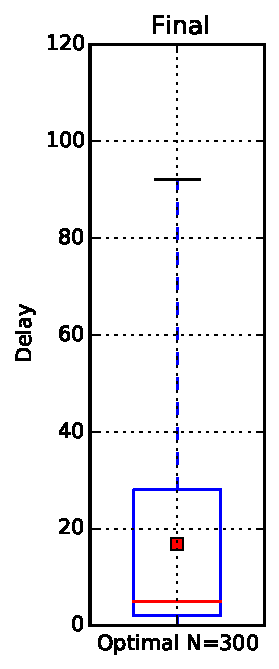
\includegraphics[keepaspectratio,height=0.3225\textwidth]{box_plot_final_9l.pdf}}
%
\caption{Increase in the total travel time w.r.t.~the optimal solution as a
function of \Nn (Figures a, c, and e) and distribution of the total delay of
each car for different values of \Nn (Figures b, d, and f).
%
For each row, the Roman numeral on top of the box plots corresponds to point the 
travel time plot marked with the same numeral.
%
The mean of the total delay is presented as a red square in box plots.
%
Plots in the $i$-th row correspond to the results for the $i$-th network in
\cref{fig:networks}.}
\label{fig:results}
\end{figure*}


%We compare the performance of non-homogeneous and homogeneous solutions in two
%ways: comparing the decrease in total travel time with increasing major frame
%time (greater look ahead), and analysing the distribution of delay in each
%queue of the network.
%
\cref{subfig:travel_time_3,subfig:travel_time_6,subfig:travel_time_9} show, for
each network, the increase in the total travel time w.r.t.~the optimal solution
as a function of \Nn.
%
As we hypothesized, the non-homogeneous discretization requires less time
intervals (i.e., smaller \Nn) to obtain a solution with the same total travel
time.
%
This is important because the size of the MILP, including the number of binary
variables, scales linearly with \Nn; therefore, the non-homogeneous approach can
scale up better than the homogeneous one (e.g., \cref{subfig:travel_time_9}).
%
Also, for homogeneous and non-homogeneous discretizations, finding the optimal
solution of major frames with large \Nn might require more time than our imposed
3000s time cutoff and, in this case, Gurobi returns a feasible control plan that
is far from optimal.
%
The effect in the total travel time of these poor solutions can be seen in
\cref{subfig:travel_time_9} for $\Nn > 120$.



The distribution of the total delay observed by each car while traversing the
network is shown in \cref{subfig:delay_3,subfig:delay_6,subfig:delay_9}.
%
Each group of box plots represents a different value of~\Nn: when the
non-homogeneous $\DT[]$ first converges; when the homogeneous~$\DT[]$ first
converges; and the optimum solution itself.
%
In all networks, the quality of the solution obtained using non-homogeneous
$\DT[]$ is better or equal than using homogeneous $\DT[]$ for fixed \Nn in both
the total travel time and \emph{fairness}, i.e., smaller third quartile and
maximum delay.

%\remark{FWT: In the paragraphs above, we need to address network 2 because it is
%the exception in both cases: in the end of \cref{subfig:travel_time_6},
%homogeneous is better, and the homogeneous delay in \cref{subfig:delay_6} is
%also better.}


\begin{figure*}[t!]
\centering

%  trim={<left> <lower> <right> <upper>}
\subfigure[]{
\label{subfig:cumu1}
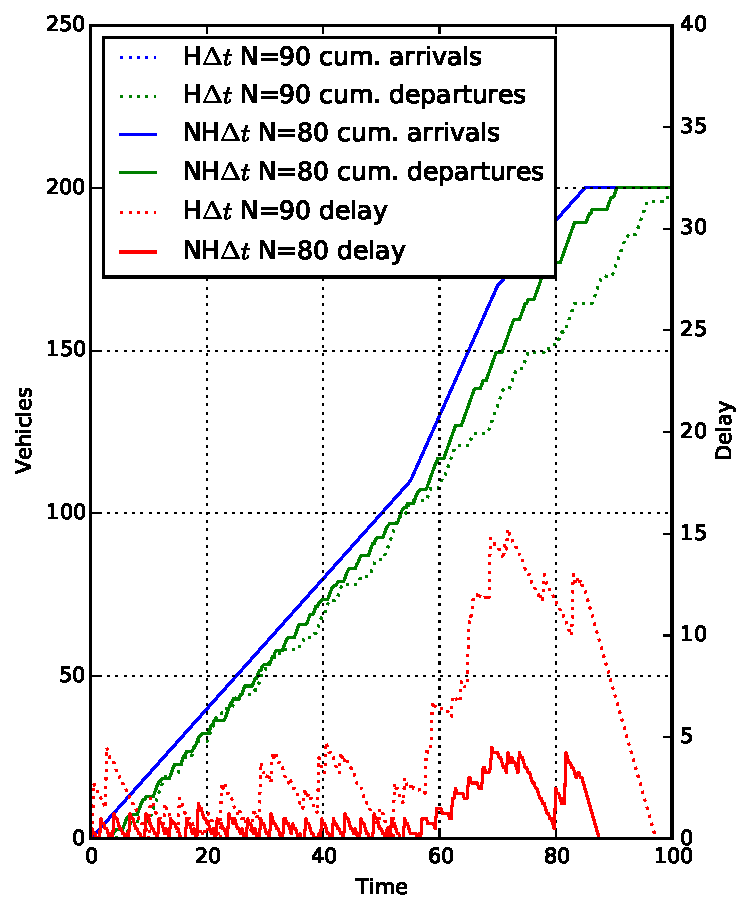
\includegraphics[width=0.32\textwidth]{cum_plot_early_6l.pdf}}
\subfigure[]{
\label{subfig:cumu2}
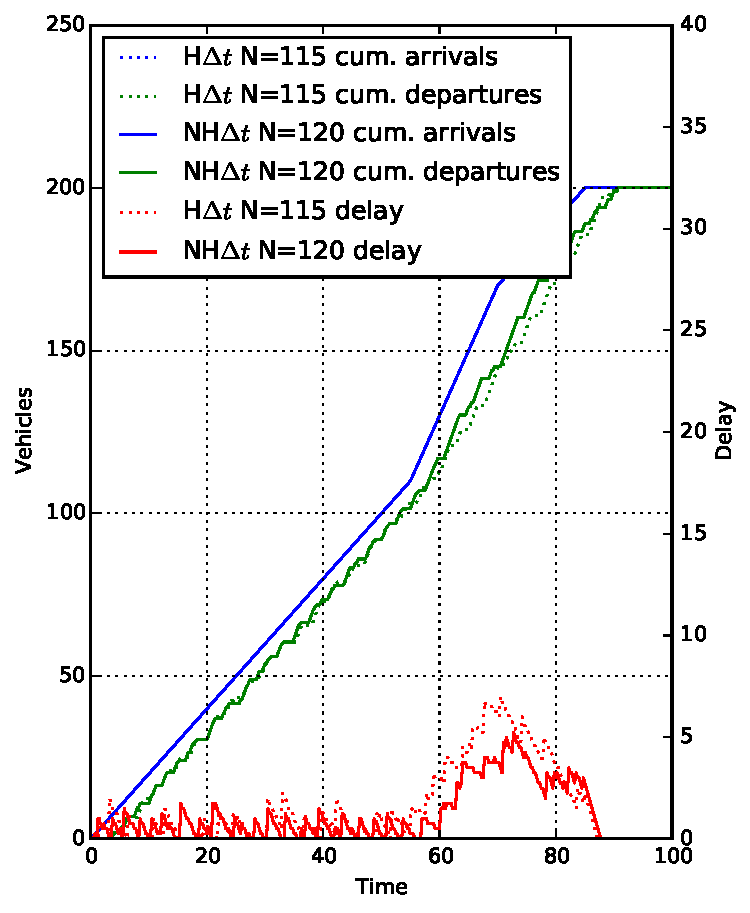
\includegraphics[width=0.32\textwidth]{cum_plot_converg_6l.pdf}}
\subfigure[]{
\label{subfig:cumu3}
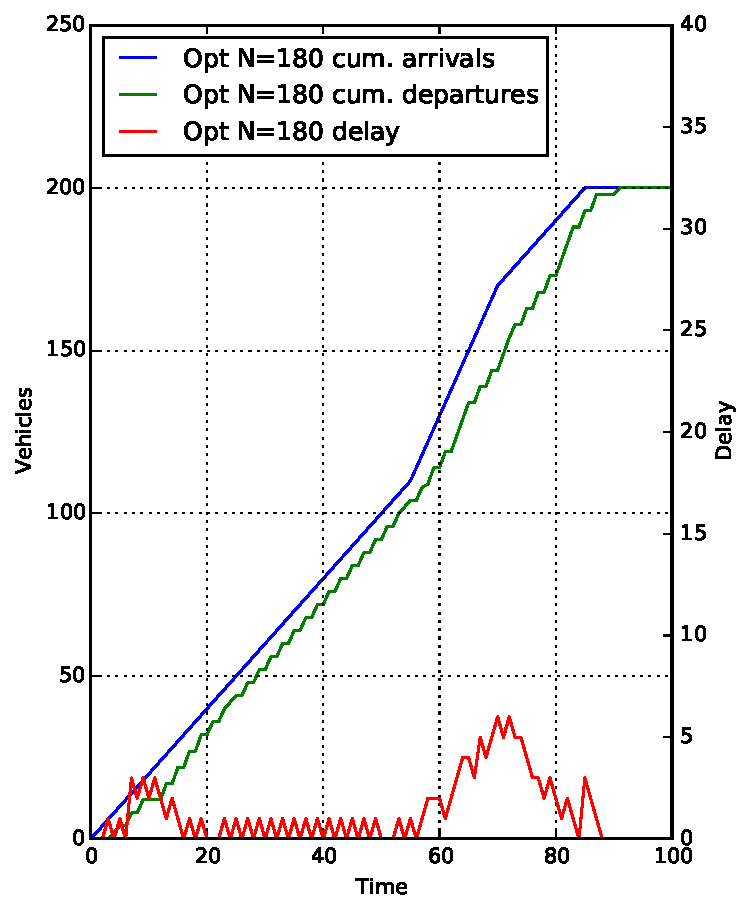
\includegraphics[width=0.32\textwidth]{cum_plot_final_6l.pdf}}
%
\caption{Cumulative arrival and departure curves and delay for queue 1 in the
2-by-3 network (\cref{subfig:network2}).
%
The value of \Nn in plots (a) and (b) corresponds, respectively, to the
convergence point of the non-homogeneous and homogeneous approaches
(\cref{subfig:travel_time_6}).
%
(c)~presents the same curves for the optimal solution.}
%
\label{fig:cumu}
\end{figure*}


To further illustrate the differences between homogeneous and non-homogeneous
discretizations, \cref{fig:cumu} shows the cumulative arrival and departure
curves and the how delay evolves over time for $q_1$ of network 2
(\cref{subfig:network2}).
%
In \cref{subfig:cumu1}, the comparison is done when non-homogeneous $\DT[]$
first converges (i.e., point I in \cref{subfig:travel_time_6}) and for this
value of \Nn, the major frame size in seconds of the non-homogeneous approach is
19.125s longer than the homogeneous one.
%
This allows the MILP solver to ``see'' 19s further in the future when using
non-homogeneous discretization and find a coordinated signal policy along the
avenue to dissipate the extra traffic that arrives at time 55s.
%
The shorter major frame of the homogeneous discretization does not allow the
solver to adapt this far in advance and its delay observed after 55s is much
larger than the non-homogeneous one.
%
Once the homogeneous $\DT[]$ has converged (\cref{subfig:cumu2}), it is also
able to anticipate the increased demand and adapt well in advance and both
approaches generate solutions close to optimum (\cref{subfig:cumu3}).


%% The related work is integrated in the introduction
%\section{Related Work}

\remark{Need a related work section with separate sections discussing
  traffic flow models and MILP-based control... suggest putting at end of article
  since we don't want reviewers to focus on this section in their comments 
  (which they would do if we put it after the introduction).}



\section{Conclusion}

In this paper, we show how our optimized adaptive traffic signal control method
based on Mixed Integer Linear Programming (MILP) can be used for mitigating the
impact of installing light rail on conventional traffic networks.
%
Our experiments show that our method is able to minimize the impact on the
average delay with respect to fixed-time signal control and also finds better
quality solutions, i.e., solutions with substantially lower third quartile and
maximum observed delay.
%
%key results show that while there is a substantial impact of light rail on
%conventional vehicle traffic delay using popular fixed-time signal control, our
%novel optimized \authorHighlight{adaptive} signal control virtually nullifies
%this impact.
%
Ultimately this leads to a win-win situation where both conventional vehicle
traffic and light rail commuters benefit through the application of MILP-based
optimization.
%
%For future mention the use of the CTM in the Conclusion to consider nonlinear
%flow models... then cite 5+ CTM papers all in one \cite{...} by borrowing
%citations from the Intro discussion of the TRB paper.



\Omit{
In this paper, we showed how to formulate a novel queue transmission model (QTM)
model of traffic flow with non-homogeneous time steps as a linear program.  We
then proceeded to allow the traffic signals to become discrete variables subject
to a delay minimizing optimization objective and standard traffic signal
constraints leading to a final MILP formulation of traffic signal control with
non-homogeneous time steps.  We
experimented with this novel QTM-based MILP control in a range of traffic networks
and demonstrated that the non-homogeneous MILP formulation
achieved (i) substantially lower delay solutions, (ii) improved per-car delay distributions,
and (iii) more optimal travel times over a longer horizon 
in comparison to the homogeneous MILP formulation with the same number of binary
and continuous variables.
%% NOTE: what bothers me here is ``larger networks'' since we don't directly
%%       compare scalability of the approaches as a function of network size
%%       (i.e., on the x-axis of some graph).  -Scott
%and demonstrated that by exploiting the non-homogeneous time steps supported
%by the QTM, we are able to scale the model up to larger networks whilst maintaining the
%same quality of a homogeneous solution using more binary
%variables.
Altogether, this work represents a
major step forward in the scalability of MILP-based jointly optimized traffic
signal control via the use of a non-homogeneous time traffic models and thus helps
pave the way for fully optimized joint urban traffic signal controllers as an
improved successor technology to existing signal control methods.
}

%We have demonstrated that by exploiting the non-homogeneous time steps
%supported by the QTM, we are able to scale the model up to larger
%networks and using the same number of binary variables as a
%homogeneous time step, and with the same quality of a homogeneous
%solution using more binary variables.


%%% Telling texcount to ignore the acknowledgment in the word counting
%TC:ignore
\section*{Acknowledgment}

%% FWT: This is the acknowledgment that the traffic group is supposed to use
%
This work is part of the Advanced Data Analytics in Transport programme, and
supported by National ICT Australia (NICTA) and NSW Trade~\&~Investment. NICTA is
funded by the Australian Government through the Department of Communications and
the Australian Research Council through the ICT Centre of Excellence Program.
NICTA's role is to pursue potentially economically significant ICT related
research for the Australian economy. NSW Trade~\&~Investment is the business
development agency for the State of New South Wales.
%TC:endignore


%% Flushing everything to have the bibliography in its own page. Some of these
%% \newpage will redundant at some point
%\begin{figure*}[t!]
%\centering
%\subfigure[]{
%\label{subfig:microsim_rail_f}
%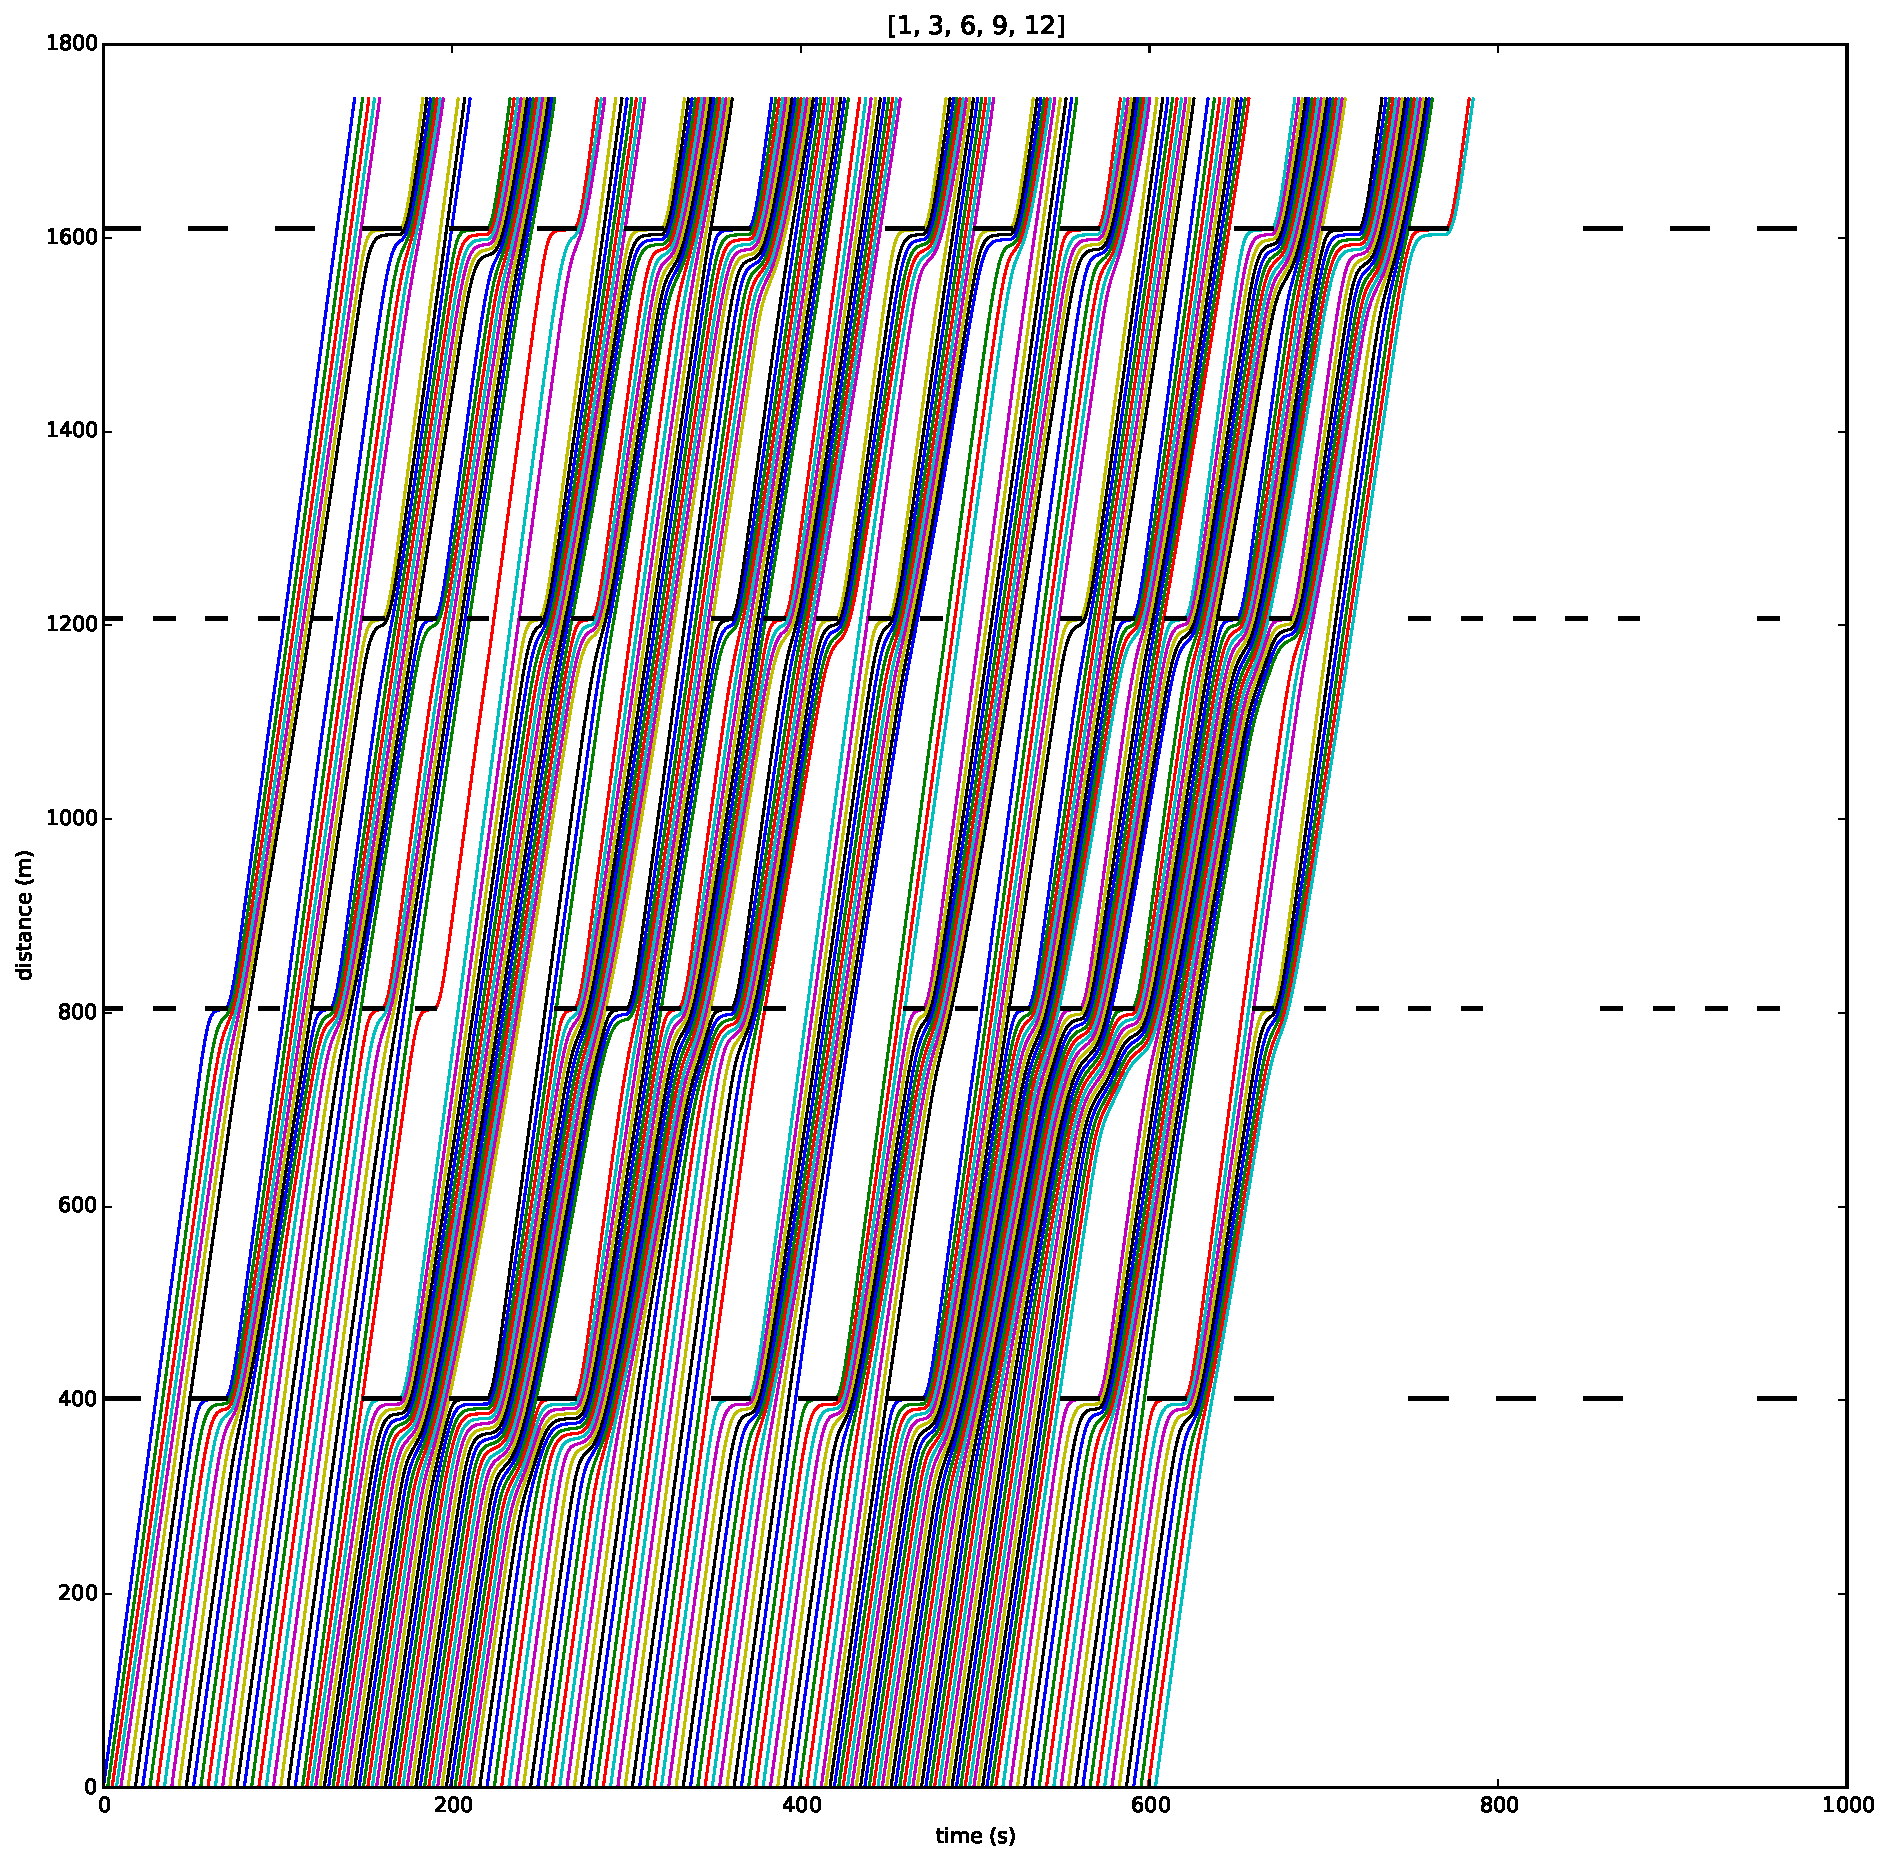
\includegraphics[width=0.49\textwidth,trim={0cm 0cm 0cm 0cm},clip]{plot_avenue_1_f_1w2.pdf}}
%\subfigure[]{
%\label{subfig:microsim_rail}
%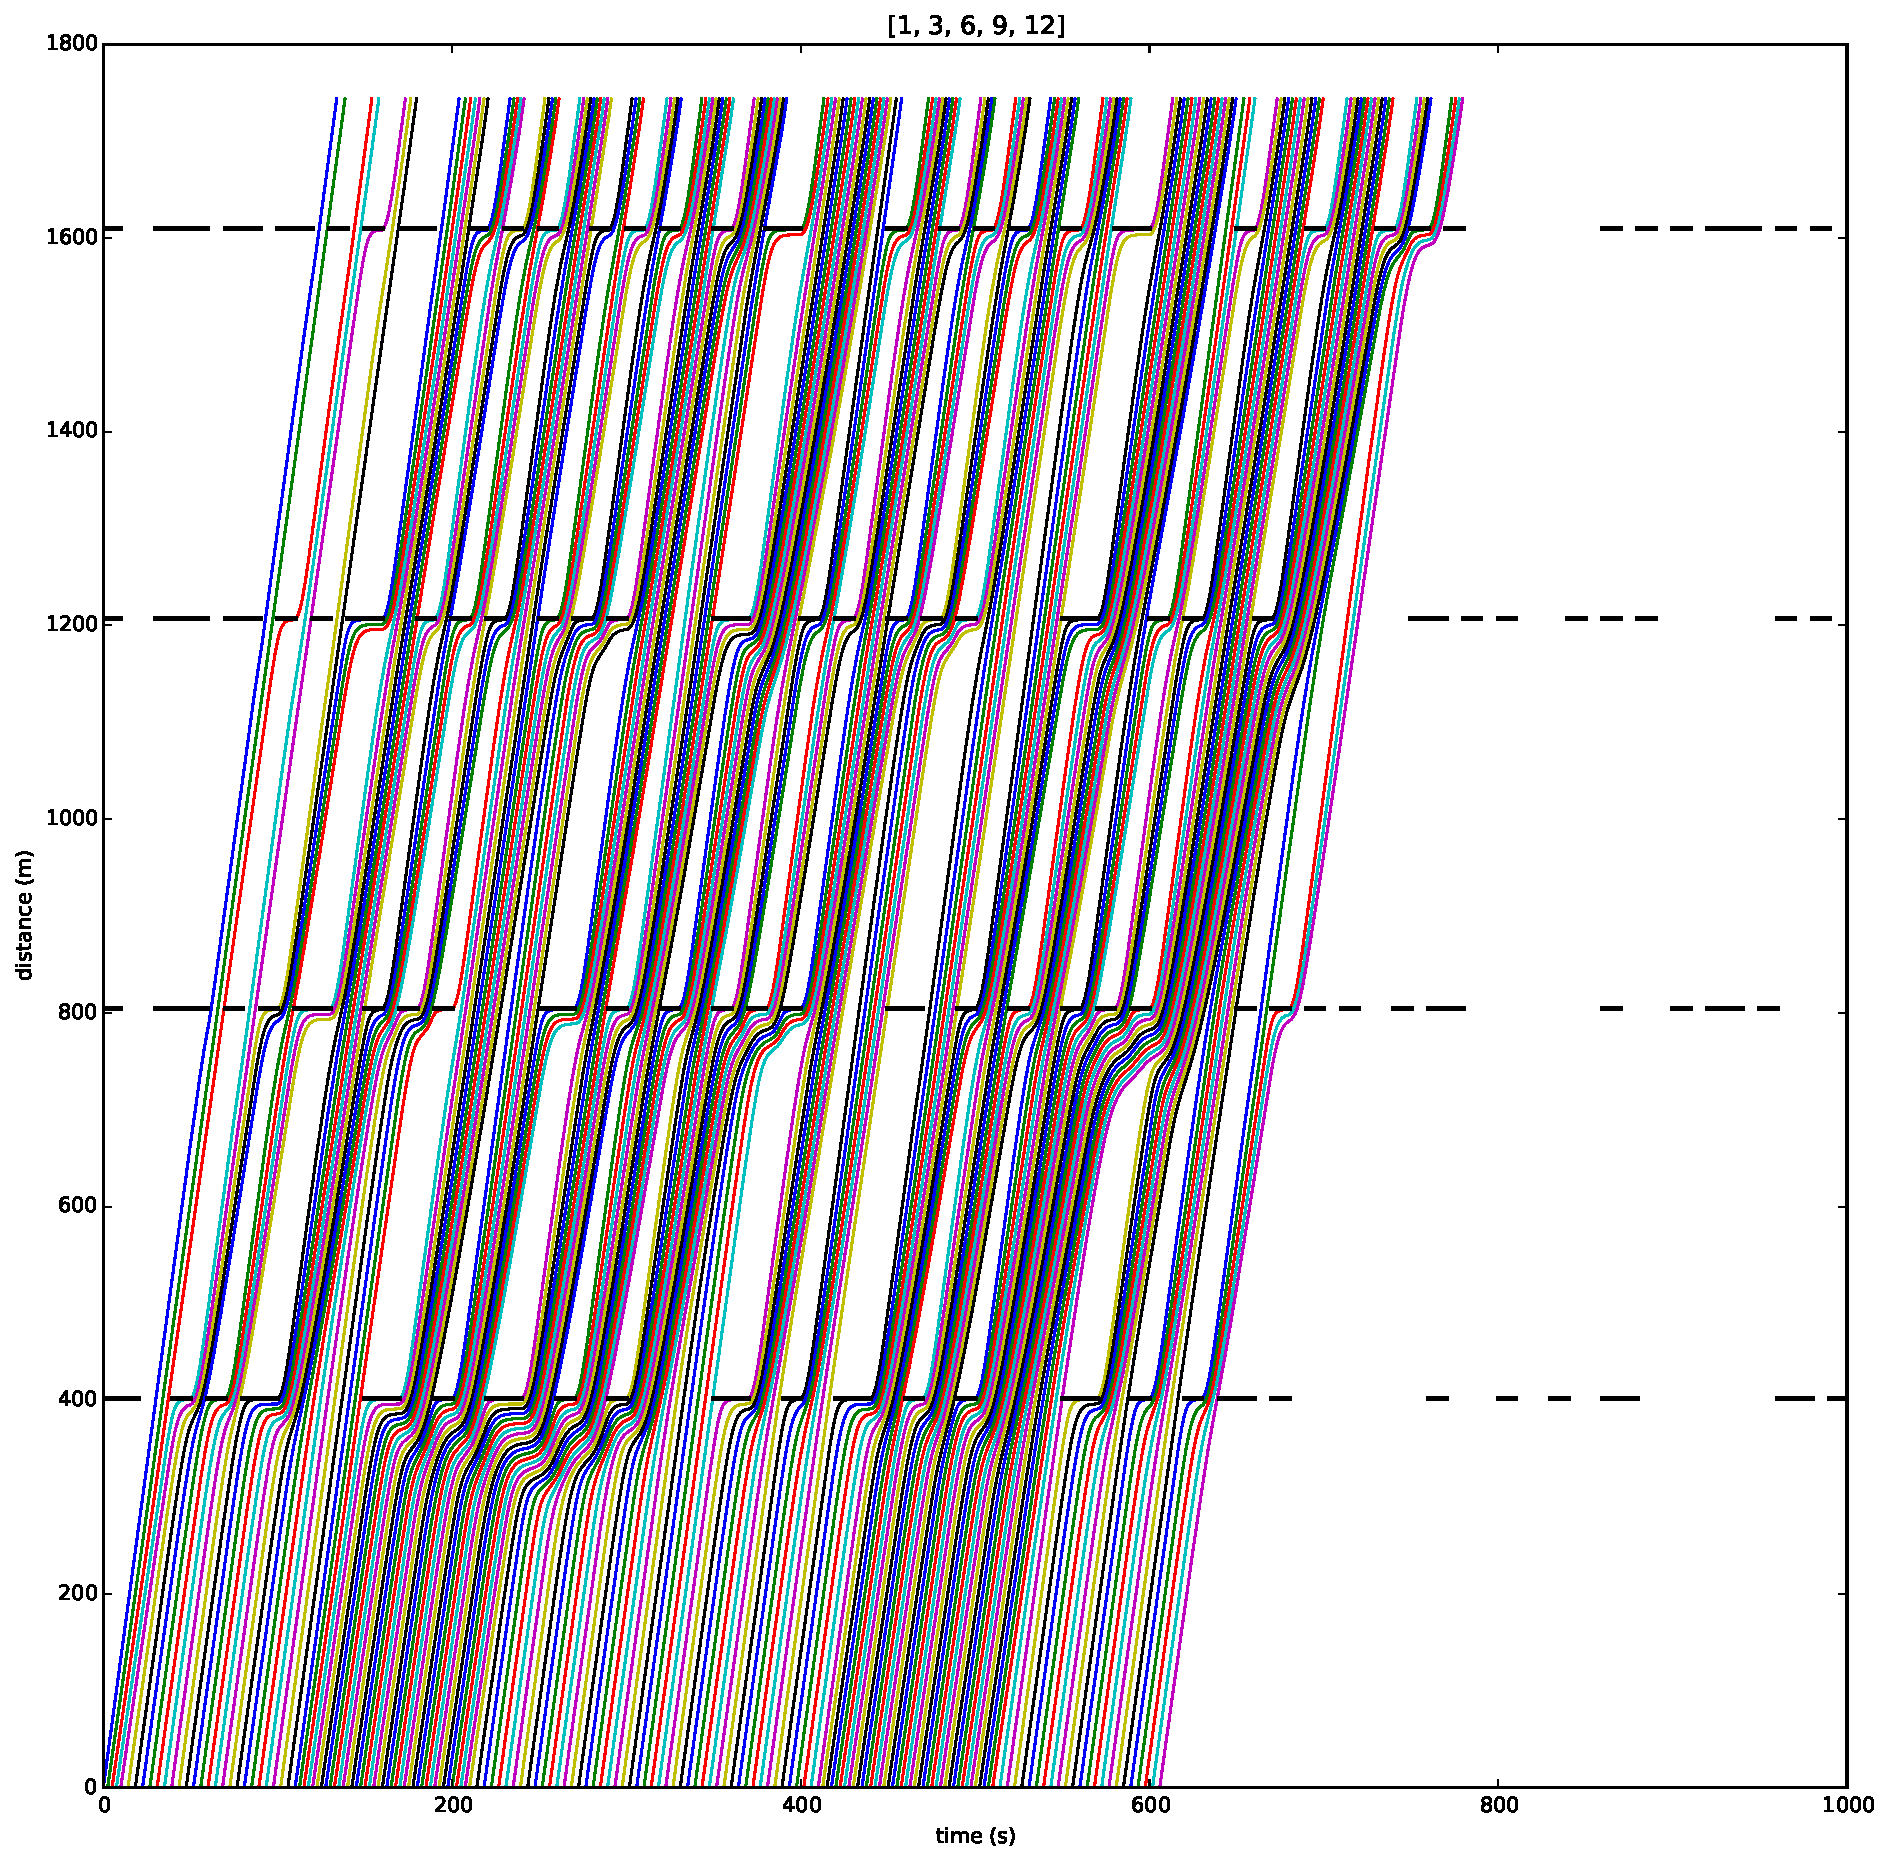
\includegraphics[width=0.49\textwidth,trim={0cm 0cm 0cm 0cm},clip]{plot_avenue_1_1w2.pdf}}
%\subfigure[]{
%\label{subfig:microsim_rail_f_side}
%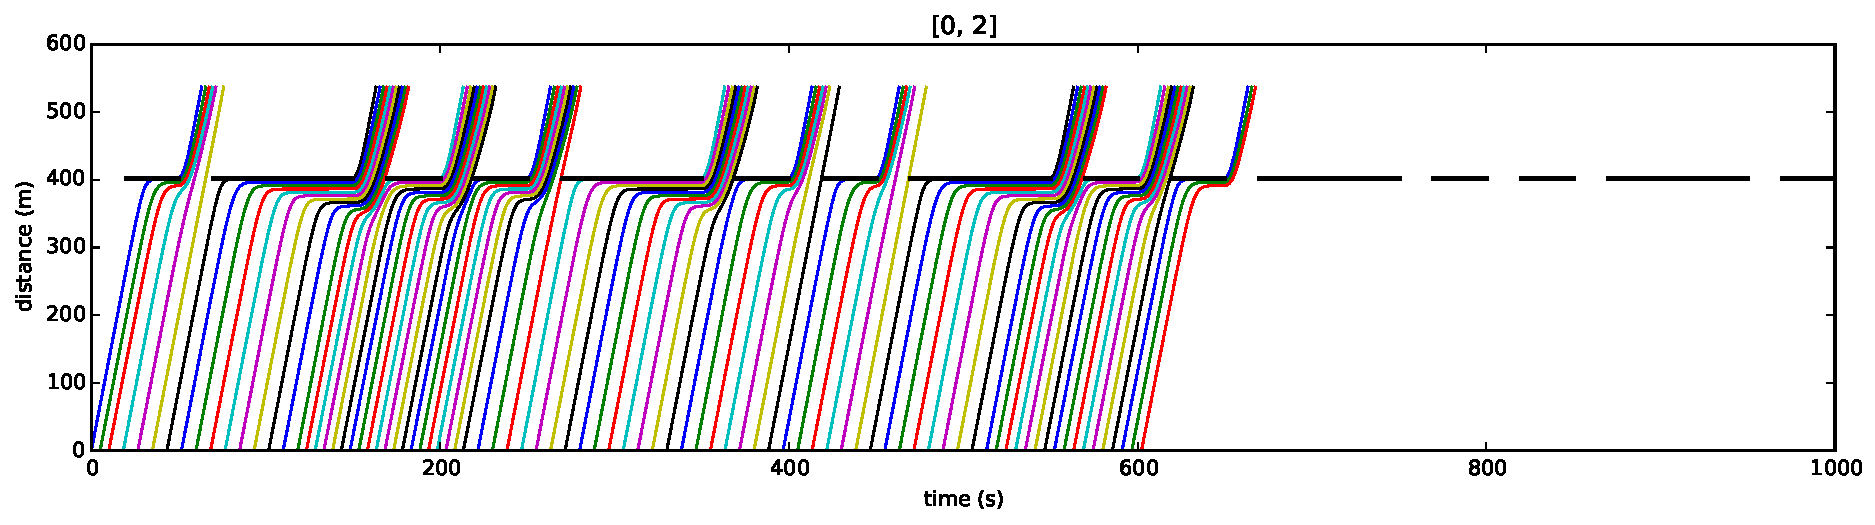
\includegraphics[width=0.49\textwidth,trim={0cm 0cm 0cm 0cm},clip]{plot_avenue_1_f_1w2_side_0.pdf}}
%\subfigure[]{
%\label{subfig:microsim_rail_side}
%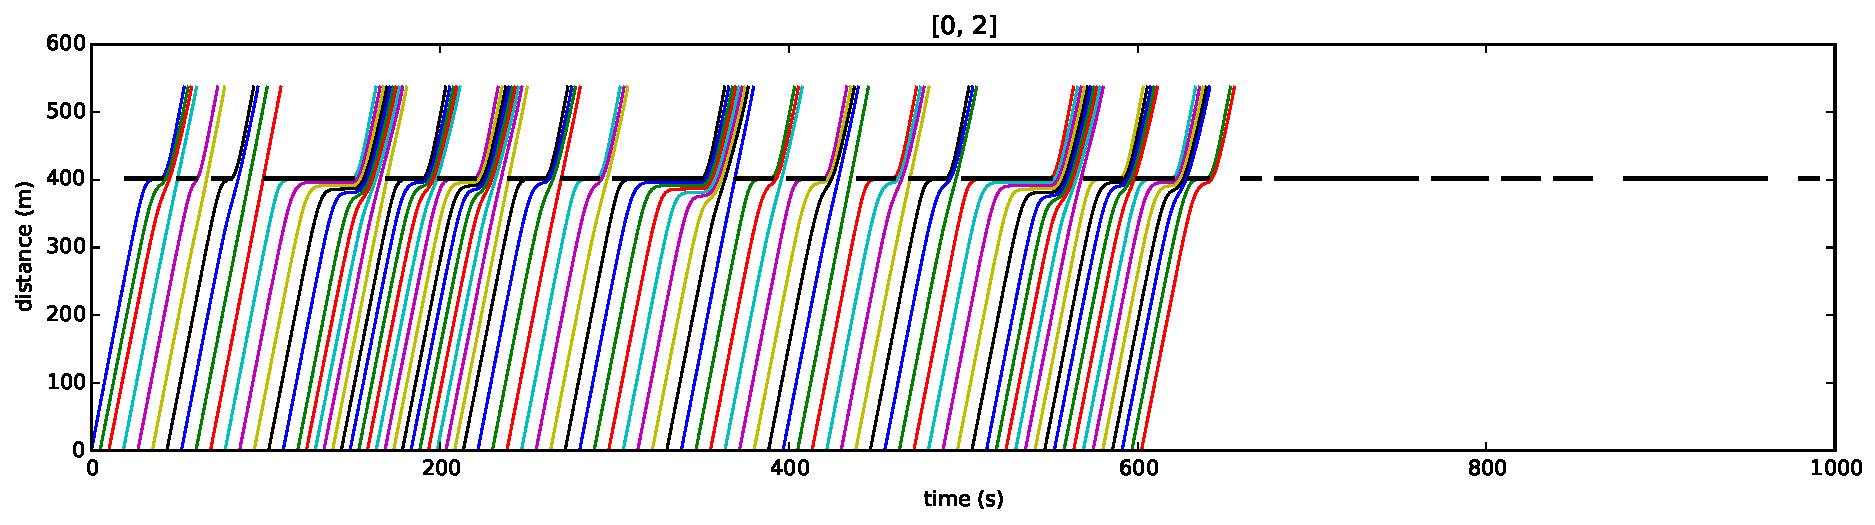
\includegraphics[width=0.49\textwidth,trim={0cm 0cm 0cm 0cm},clip]{plot_avenue_1_1w2_side_0.pdf}}
%\label{fig:micosim}
%\end{figure*}

%\newpage
%~
%\newpage
%~
%\newpage



\bibliographystyle{aaai}
\bibliography{Transport}


\end{document}
